\documentclass[11pt, a4paper,oneside,chapterprefix=false]{scrbook}

% setup with overleaf
\usepackage{a4wide}
\usepackage{times}
\usepackage{helvet}   % sets sans serif font
\usepackage{algorithm}
\usepackage{algpseudocode}
\usepackage{amsmath,amssymb,amsthm}
\usepackage{svg}
\usepackage{graphicx}
\usepackage{subfigure}  
\usepackage{fancybox} % for shadowed or double bordered boxes
\usepackage{fancyhdr}
\usepackage{float}
\usepackage{cite}
\usepackage{listings}
\usepackage[colorlinks=true, allcolors=black]{hyperref}
\usepackage{xargs}
\usepackage{pgfplots}
\usepackage[colorinlistoftodos,prependcaption,textsize=tiny]{todonotes}


\newcommand{\todochange}[2][1=]{\todo[linecolor=blue,backgroundcolor=blue!25,bordercolor=blue,#1]{#2}}

\DeclareGraphicsExtensions{.pdf,.jpg,.png}

%% macros
\input{include/math}
\input{include/codelisting_layout}

\usepackage{color}
\definecolor{RED}{rgb}{1,0,0}
\definecolor{GREEN}{rgb}{0,0.7,0}
\definecolor{BLUE}{rgb}{0,0,1}
\newcommand{\FIXME}[1]{{\color{RED}{\textbf{FIX}: #1}}}

\addtolength{\textheight}{2.0cm}
\addtolength{\voffset}{-1cm}
\addtolength{\textwidth}{1.8cm}
\addtolength{\hoffset}{-.9cm}

\widowpenalty=10000
\clubpenalty=10000

\lstdefinelanguage{json}{
    basicstyle=\small\ttfamily,
    numbers=left,
    numberstyle=\scriptsize,
    stepnumber=1,
    numbersep=6pt,
    showstringspaces=false,
    breaklines=true,
    frame=lines,
    backgroundcolor=\color{background},
    stringstyle=\color{string},
    keywordstyle=\color{keyword},
    commentstyle=\color{comment},
    morecomment=[l]{//},
    morecomment=[s]{/*}{*/},
    morecomment=[l]{\#},
    morestring=[b]",
    morestring=[b]',
    morekeywords={true,false,null}
}

\definecolor{background}{HTML}{EEEEEE}
\definecolor{keyword}{RGB}{170,85,0}
\definecolor{string}{RGB}{0,128,0}
\definecolor{comment}{RGB}{128,128,128}


\begin{document}

\frontmatter
%\maketitle %automatic version
% --- selfmade version ----
\begin{titlepage}
	\setlength{\parindent}{0cm}
	\addtolength{\textheight}{1.0cm}

	\vspace{0.2cm}
	\Huge
	\begin{center}
		{\textsf{\textbf{Analyzing the Impact of Occlusion on the Quality of Semantic Segmentation Methods for Point Cloud Data}}}	
	\end{center}
	

	\vfill \vfill \vfill
	\begin{figure}[h]
		\centering
		\includegraphics*[width=1.0\textwidth]{figures/cover.png}
	\end{figure}

	\vfill
	\sffamily\Large
	\begin{center}
		{\textbf{Bachelor Thesis}} \\ 
		13th March 2023 - 13th September 2023 \\[0.5cm]
		\large
		Yufeng Xiao \\ 19-763-663
	\end{center}

	\vfill \vfill \vfill
	\begin{minipage}[b]{0.5\textwidth} \raggedright
	Supervisors: \\
	Prof. Dr. Renato Pajarola \\
	Lizeth Joseline Fuentes Perez \\
	\end{minipage}
	%
	\begin{minipage}[b]{0.5\textwidth} \raggedleft
	Visualization and MultiMedia Lab \\
	Department of Informatics \\
	University of Z{\"u}rich
	\end{minipage}

	\vfill
	\hrule
	\vspace{0.5cm}
	\includegraphics*[width=0.3\textwidth]{figures/uzh_logo} \hfill
	\includegraphics*[width=0.3\textwidth]{figures/vmml_logo}
\end{titlepage}
%%

%=====================================================================
\chapter{Abstract} \label{chp:abstract}
%=====================================================================

This thesis aims to analyze the impact of occlusion on the quality of semantic segmentation methods for point cloud data. Occlusion is a prevalent phenomenon in 3D scenes, where objects often overlap or obstruct each other. This can significantly compromise the quality and integrity of data, leading to inaccuracies in semantic segmentation. While the issue of occlusion has garnered attention in 3D data processing, current research on how different occlusion levels impact the quality of semantic segmentation is rare. Specifically, there is a palpable gap in understanding how to quantify occlusion in the scene and how this characteristic influence the performance of advanced semantic segmentation software like the Minkowski Engine. To bridge the research gap, we proposed a novel metric to quantify the occlusion level of a scene. We then applied this metric to analyze the impact of occlusion on the quality of semantic segmentation methods for point cloud data. Our results show that the occlusion level of a scene has limited impact to the quality of semantic segmentation.

\tableofcontents

\listoffigures

\lstlistoflistings

\mainmatter

%=====================================================================
\chapter{Introduction and Related Works} \label{chp:introduction}
%=====================================================================


Artificial intelligence has received significant attention in recent research. Fields such as natural language processing, image generation, and autonomous driving have benefited from considerable investments, and some related applications have been successfully implemented. Currently, the practical implementation of autonomous driving is still challenging due to the high demands for model performance and safety. To achieve its goals, AI needs to precisely understand its surrounding environment. Hence, semantic segmentation of scenes has become an essential topic. In this thesis, as opposed to focusing on outdoor scenes commonly associated with autonomous driving, we are more interested in understanding indoor environments. The correct classification and comprehension of indoor objects can assist in various aspects of human life, such as creating intelligent robots to help humans with a series of tasks. To understand scenes accurately, we need to provide AI with high-precision data, typically point clouds, which are a collection of data points defined in a three-dimensional coordinate system, represent the external surface of an object. These data points can capture the shape, and sometimes color, of the physical entities in a scanned environment. They are usually obtained from laser scanners or multi-view reconstructions. However, when collecting this type of data, objects are often obstructed due to the viewpoint of the scanner, leading to occlusions in the data, as shown in Figure \ref{fig:occlusion in a scene}, where part of occlusions in a scene are marked with red box. Therefore, we aim to explore how occlusion affects AI's understanding of a scene. More specifically, we want to propose a metric to reflect the occlusion level of a scene and analyze how this characteristic influences the performance of semantic segmentation methods.


\begin{figure}[h]
    \centering
    \includegraphics*[width=1.0\textwidth]{figures/occlusion in conf2.png}
    \caption{Occlusion in a scene}
    \label{fig:occlusion in a scene}
\end{figure}

\section{Previous work}
To the best of our knowledge currently there is not explicit works that compute occlusion level for an entire indoor scene. There are some related works handling occlusion of point cloud. In this section, we will briefly introduce these works, especially the ones that are related to occlusion.  


\paragraph{Occlusion Guided Scene Flow Estimation on 3D Point Clouds.} \label{par:scene flow}

This paper \cite{OR:21} presents the OGSF-Net, a novel architecture designed to address the challenges of occlusions in 3D scene flow estimation. Occlusions, where certain regions in one frame are hidden in another, can hinder accurate flow estimation. The OGSF-Net uniquely integrates the learning of flow and occlusions, using an occlusion handling mechanism in its Cost Volume layer to measure frame correlations. This approach aims to enhance both flow accuracy and the understanding of occluded regions, marking a pioneering effort in 3D scene flow estimation on point clouds. To make this method robust, it is important to make an accurate occlusion prediction. Therefore, they evaluate the performance of occlusion estimation on data set FlyingThings3D \cite{MIFDB16}, which provides the ground truth occlusion mask of point cloud. For evaluation, they use accuracy and F1 score as metrics. This inspires us to apply similar metrics to evaluate the result of semantic segmentation.

\paragraph{OcCo: Unsupervised Point Cloud Pre-training via Occlusion Completion.} \label{par:OcCo occlusion completion}

In this work \cite{Wang:21}, the authors proposed \emph{Occlusion Completion}, an unsupervised pre-training method. The main idea is to generate occlusion in a point cloud, then use an encoder-decoder model to reconstruct occluded points, and apply the encoder weights for downstream tasks. What is interesting for us is how they generate occlusion in a scene. They view point cloud from a camera, which is placed in different viewpoints. At each viewpoint, points are projected to a camera reference frame, if some points share the same pixel coordinates, then there might be occlusion. This could also be an inspiration for us to generate occlusion in a scene.

\section{Positioning and Contributions}

Previous work has shown that occlusion of a point cloud can be estimated based on ground truth occlusion information. However, in our work we have to estimate occlusion level of a scene without knowing such information. To achieve this, we will define occlusion as the amount of area occluded from a particular scan viewpoint. To estimate occlusion we defined, we propose the metric \emph{occluded area ratio} to represent occlusion level in the scene which is represented by a triangulated mesh. 

\vspace{10pt}

This work is focusing on the data set of point cloud. Since there is no property can quantify area in point cloud we cannot directly extend the metric \emph{occluded area ratio} to point-based data structure. Therefore, we have to use a different metric to estimate occlusion level, here we propose \emph{Boundary ray ratio} which is the ray that intersect with boundary points in point cloud. We also defined boundary points based on their semantic labels.

%=====================================================================
\section{Technical Background}
%=====================================================================

Based on the introduction in previous sections, we would elaborate on some key concepts in the technical background of this work.

\subsection{Point Cloud Data}

A point cloud is a discrete set of data points in space. The points may represent a 3D shape or object. Each point position has its set of Cartesian coordinates (X, Y, Z), in some cases it can also include color(RGB) or intensity information. Point clouds are generally produced by 3D scanners or by photogrammetry software, which measure many points on the external surfaces of objects around them. 

\vspace{10pt}

Point cloud can be used in different areas. One usage is for rendering and modeling. Typically 3D objects are modeled using polygon meshes, and  polygons are the rendering primitives in the graphics pipeline. However, representing all objects with point sampling allows easy mixing of objects in a scene without specialized algorithms for different geometry types. Other applications include depth sensing, perception, scientific computing etc.

\subsection{Semantic Segmentation}

Semantic segmentation for point cloud data has rapidly became a pivotal research domain, given its profound implications in many applications. From the intricate pathways navigated by autonomous driving to the precise movements of robotics and the detailed analysis of 3D scenes, the ability to accurately segment and categorize each data point in a 3D environment is important.

\vspace{10pt}

At the heart of this research lies the challenge of dealing with occlusions. In real-world scenarios, objects within a scene often overlap or obstruct each other, leading to partial or even complete occlusions. Such occlusions can significantly distort the spatial distribution of data points, making it challenging to distinguish the structure and category of the obstructed objects. For instance, in an urban driving scenario, a pedestrian might be partially hidden behind a parked car, or in an indoor scene, a chair might be obscured by a table. These occlusions can lead to misclassifications, reducing the overall accuracy of the segmentation.


\paragraph{Minkowski Engine.}

The Minkowski Engine \cite{CGS:19} is an auto-differentiation library specifically designed for sparse tensors. In the area of deep learning, where dense tensors are commonly used, the Minkowski Engine brings a fresh perspective by focusing on sparse tensors. This is particularly beneficial for 3D data, which often exhibits spatial sparsity. The engine supports all standard neural network layers, including convolution, pooling, unpooling, and broadcasting operations, but tailored for sparse tensors. Such capabilities make it an ideal choice for semantic segmentation tasks, especially when dealing with point cloud data. [Minkowski]

\begin{figure}[h]
    \centering
    \includegraphics*[width=0.75\textwidth]{figures/Minkowski Engine.png}
    \caption{Minkowski Engine Indoor Scene Segmentation}
    \label{fig:minkowski}
\end{figure}


\section{Motivation} \label{sec:motivation}

Among the many factors influencing the semantic segmentation of point cloud data, the level of occlusion stands as one of the major challenges. Occlusions, a prevalent phenomenon in 3D scenes, can significantly compromise the quality and integrity of data. When objects are partially or entirely obscured by others, semantic segmentation might lead to inaccuracies in segmentation. While the issue of occlusion has garnered attention in 3D data processing, current research on how different occlusion levels impact the quality of semantic segmentation remains fragmented. Specifically, there is a palpable gap in understanding how to quantify occlusion levels and how these levels influence the performance of advanced tools like the Minkowski Engine. Thus, the primary motivation behind this research is to systematically evaluate level of occlusion and delve deep into their impact on point cloud data semantic segmentation.

\section{Outline} \label{sec:outline}

In this thesis we will first briefly mention related works and discuss the part which bring us inspirations. We will also introduce related technical concepts to give reader richer background information. Then our contributions and motivations will be stated. In the next Chapter we elaborate on problems which we have to solve in order to compute metrics proposed before correctly. Our technical solution are listed and explained in detail with figures and formulas in Chapter \ref{chp:solution}. Once we have the solution, we will start to implement concrete codes. Thus, in Chapter \ref{chp:implementation} implementation details of our algorithm are explained together with the technical stack applied to support our computational pipeline. In the end of this part we will introduce the structure of our software to give insights on how the whole pipeline works.

\vspace{10pt}

For this thesis it is crucial to present our experimental results in a meaningful way. Hence, in Chapter \ref{chp:experimental results} we need to first validate that those metrics we proposed can accurately reflect the level of occlusion of a point cloud. With successful validation we can then apply them to correlate with the performance of semantic segmentation. In the final step, we discuss the result of experiments and conclude this thesis.


%=====================================================================
\chapter{Problem Statement} \label{chp:problem}
%=====================================================================

In this thesis we aim to find the correlation between occlusion level and performance of semantic segmentation. Given a data set include mesh and point cloud, we have to first prove that \emph{occluded area ratio} can be computed correctly in a mesh. To extend this metric to point cloud, we would estimate a mesh from the cloud and we compute its occluded area ratio. Then we would directly generate a set of occluded point clouds to apply the \emph{Boundary ray ratio} to estimate level of occlusion. To validate \emph{Boundary ray ratio} is a reliable metric in estimation, its value should be close to the value of \emph{occluded area ratio}. After the validation we can compute occlusion level of point cloud together with the performance of semantic segmentation, then we compare performance of point cloud with different occlusion level to see if these metrics can correlated with each other.

\vspace{10pt}

These problems are addressed in following points. Each of them will be provided with more detailed explanation in the next chapter where our technical solutions are given.

\begin{itemize}
    \item Compute \emph{occluded area ratio} of mesh.
    \item Estimate a mesh from the given point cloud.
    \item Compute the \emph{occluded area ratio} for the estimated mesh and generate a new point cloud from the visible area of the mesh.
    \item Apply the \emph{Boundary ray ratio} metric to the new point cloud to estimate the level of occlusion and validate the reliability of the \emph{Boundary ray ratio} metric by comparing its value with the \emph{occluded area ratio}
    \item Compute the occlusion level and the performance of semantic segmentation of the point cloud, then compare these metrics between different clouds to find correlation. 
\end{itemize}


\section{Occluded Area Ratio of Mesh} \label{sec:occluded area ratio of mesh}

In this part we have to prove that as the number of viewpoints increase, there will be more visible area. In another word, there is less occluded region and thus lower occlusion. As shown in figure \ref{fig:scene with light sources}, which is generated by simulating a scene with multiple light sources in blender \cite{blender2023}, the scene with 2 viewpoints has more bright area and less shadow, this also matches our intuition in real life. 

\vspace{10pt}

To determine which area is visible and which is not is the key point here to compute occluded area ratio correctly. Obviously, the visible region to a viewpoint is where rays from viewpoint can reach. Hence, ray-tracing based algorithm will play an important role in computation of occlusion level.  

\begin{figure}[H]
    \centering
    \subfigure[1 viewpoint]{\includegraphics[width=0.8\textwidth]{figures/1 vp.png} \label{fig:1 vp}} \hfill
    \subfigure[2 viewpoints]{\includegraphics[width=0.8\textwidth]{figures/2 vp.png} \label{fig:2 vp}}
    \caption{Scene with Light Sources}
    \label{fig:scene with light sources}
\end{figure}

\section{Mesh Estimation from Point Cloud} \label{mesh estimation of point cloud}

If we want to compute \emph{occluded area ratio} from a point cloud, we have to first generate mesh from it. This mesh is certainly only an estimation. Algorithm such as region growing \cite{pcl_tutorial_2023_rg} can segment points into clusters based on their properties. With these clusters we can estimate a plane for each of them, then we have a mesh composed by a set of planar primitives. The accuracy of estimation in this step will also affect subsequent process, hence, it is crucial for us to improve the result of mesh estimation. 

\vspace{10pt}

In case of region growing, we need to tweak its input parameters. An example of a code snippet is shown in List \ref{lst:region_growing}, with many parameters to adjust, the result of region growing can be unstable, which also makes subsequent process difficult to control. Therefore, it is essential to find a more accurate way to estimate mesh.   
\begin{lstlisting}[language=C++, caption=Region Growing, label=lst:region_growing]
    pcl::RegionGrowing<pcl::PointXYZ, pcl::Normal> reg;
    reg.setMinClusterSize(min_cluster_size);
    reg.setMaxClusterSize(max_cluster_size);
    reg.setSearchMethod(tree);
    reg.setNumberOfNeighbours(num_neighbours);
    reg.setInputCloud(cloud);
    reg.setInputNormals(normals);
    reg.setSmoothnessThreshold(smoothness_threshold / 180.0 * M_PI);
    reg.setCurvatureThreshold(curvature_threshold);
    reg.extract(rg_clusters);
\end{lstlisting}

\section{Generate Point Cloud from Estimated Mesh} \label{generate point cloud from estimated mesh}

Once we have a mesh, we can directly generate points from each face of it. One way to do that is sampling points on polygon, which is normally triangle. We have to make the distribution of points as uniform as possible so that the structural information of mesh can be kept precisely. Otherwise, the generated point cloud will give us distorted information which may lead to significantly biased result of computation. The other way to have points from mesh could be related to ray in the scene. As we mentioned in section \ref{sec:occluded area ratio of mesh}, ray-tracing based mesh can be applied to our pipeline. When there is ray in the scene, we can compute intersections between ray and triangle. These intersections can present structural information of mesh as well, in case of first hit intersection point, we know that the region surrounding this point is visible. This information of visibility may contribute to subsequent computations. 


\section{Boundary Ray Ratio of Point Cloud}

A common way to generate point cloud is conducted by casting lasers from scanner. Since lasers cannot pass through objects, occlusion is then generated on those obscured surfaces. And they are mostly shown on the exterior structure of an indoor scene such as walls, floors and ceilings etc, as they are located in the outermost layer of the room. Items such as chairs and tables, they can also be obscured by other things, but it is difficult to estimate how much they are occluded since their structure is more complex compared to large structures like walls. An example of exterior and interior structure of point cloud is shown in Figure \ref{fig:Exterior and interior structure of a point cloud}.

\begin{figure}[H]
    \centering
    \subfigure[Exterior]{\includegraphics[width=0.65\textwidth]{figures/conf2 ext.png}} \label{fig:exterior} 
    \subfigure[Interior]{\includegraphics[width=0.65\textwidth, height=0.4\textwidth]{figures/conf2 int.png}} \label{fig:interior}
    \caption{Scene with Light Sources}
    \label{fig:Exterior and interior structure of a point cloud}
\end{figure}

\vspace{10pt}

Based on what we stated above, we choose \emph{Boundary ray ratio} as the metric to estimate occlusion in point cloud. A set of rays will be cast to detect if it intersect with points identified as exterior structure, in this work we define these external points as boundary. With ground truth labeling of points, the classification of points can easily be done. Finally, we can compute a ratio related to ray that intersects boundary to represent occlusion level of a point cloud. 

\section{Performance Evaluation of Semantic Segmentation} \label{sec:performance evaluation}

This step is to find correlation between occlusion level and performance of semantic segmentation. From previous steps we can already compute occlusion level of a point cloud. The problem here is to use some metrics to evaluate the performance of segmentation. In Section \ref{par:scene flow}, the author of the related work about scene flow, applied F1 score to evaluate their results. This will be considered as one of the options for evaluation. With metrics we computed before we can finally investigate how would the evaluation metrics change with different occlusion level. 

%=====================================================================
\chapter{Technical Solution} \label{chp:solution}
%=====================================================================

In this chapter we will introduce our technical solution to the problem stated in Chapter \ref{chp:problem} in a detailed way. The overall workflow is shown below in Figure \ref{fig:overall flowchart of technical solution}.

\begin{figure}[H]
    \centering
    \includegraphics*[width=0.38\textwidth]{figures/technical solution flowchart.png}
    \caption{Overall Flowchart of Technical Solution}
    \label{fig:overall flowchart of technical solution}
\end{figure}

\section{Compute Occluded Area Ratio} \label{sec:compute occluded area ratio}

It is difficult to accurately compute occluded area of a triangle, since we don't exactly know which part is visible or occluded geometrically. The method applied here is to sample triangle, with samplings we can have a good coverage of the area. Next step is to compute each sampling's visibility to viewpoints in the scene. Then we are able to compute the ratio by counting how many points are occluded. A flow chart of the whole pipeline is shown below in Figure \ref{fig:flowchart of computing occluded area ratio}.

\begin{figure}[H]
    \centering
    \includegraphics*[width=1.0\textwidth]{figures/Compute occluded Area Ratio.png}
    \caption{Flowchart of Computing occluded area ratio}
    \label{fig:flowchart of computing occluded area ratio}
\end{figure}

\subsection{Sample Triangles} \label{subsec:sample triangle}

In order to make samplings cover the area of triangle uniformly, we take 2 sampling algorithms into consideration. There are uniform sampling and halton sampling. The only difference of these methods is the way they generate random numbers. With these number we calculate barycentric coordinates based on vertices of triangle. 

\paragraph{Uniform Sampling}

The process begins by randomly generating two parameters, \( r_1 \) and \( r_2 \), both of which lie in the interval [0, 1] with a uniform distribution, ensuring that each point within the interval has an equal probability of being selected. These random parameters are then used to compute the barycentric coordinates of the sampled points within the triangle. The barycentric coordinates, denoted as \( \alpha \), \( \beta \), and \( \gamma \), allow us to express any point within the triangle as a linear combination of the triangle's vertices.

\vspace{10pt}

The algorithm of this part is shown below: 

\begin{algorithm}
\caption{Uniform Sampling within a Triangle}\label{alg:uniform_sampling}
\begin{algorithmic}
\Require Triangle vertices \(V_1\), \(V_2\), \(V_3\)
\Ensure Sampled point \(P\) within the triangle
\State Generate two random numbers \(r_1\) and \(r_2\) with a uniform distribution in the interval [0, 1]
\State Compute the barycentric coordinates using \(r_1\) and \(r_2\) as follows:
\State \hspace{0.5cm} \( \alpha \gets 1 - \sqrt{r_1} \)
\State \hspace{0.5cm} \( \beta \gets \sqrt{r_1} \times r_2 \)
\State \hspace{0.5cm} \( \gamma \gets 1 - \alpha - \beta \)
\State Compute the Cartesian coordinates of the sampled point \(P\) as:
\State \hspace{0.5cm} \( P \gets \alpha V_1 + \beta V_2 + \gamma V_3 \)
\State \Return \(P\)
\end{algorithmic}
\end{algorithm}


\paragraph{Halton Sampling}

In the part of uniform sampling, we have introduced how to compute barycentric coordinates on a triangle. Therefore, here we focus on the generation of random numbers using the Halton sequence, a method that generates quasi-random numbers which are known to fill the space more uniformly compared to purely random numbers.

\vspace{10pt}

The algorithm to generate a number in the Halton sequence can be represented as:

\begin{algorithm}[H]
\caption{Halton Sequence Generation}\label{alg:halton}
\begin{algorithmic}
\Require $index \geq 0$, $base > 1$ (a prime number)
\Ensure Halton number corresponding to the given index and base
\State $result \gets 0.0$
\State $f \gets 1.0 / base$
\State $i \gets index$
\While{$i > 0$}
    \State $result \gets result + f \cdot (i \mod base)$
    \State $i \gets i / base$  \Comment{Integer division}
    \State $f \gets f / base$
\EndWhile
\State \Return $result$
\end{algorithmic}
\end{algorithm}


Using this method, we generate two sequences of Halton numbers with different bases such as 2 and 3, respectively, which are then used to compute the barycentric coordinates for uniform sampling within a triangle. These quasi-random numbers, \( r1 \) and \( r2 \), provide a more evenly distributed set of sample points within the triangle compared to purely random sampling, facilitating a more uniform sampling process. This can be verified in Figure \ref{fig:sample triangle}, where halton sampling shows a result which is closer to even distribution.  

\begin{figure}[H]
    \centering
    \subfigure[Uniform]{\includegraphics[width=0.7\textwidth]{figures/uniform sample triangle.png}}  \label{fig:uniform sampling} 
    \subfigure[Halton]{\includegraphics[width=0.7\textwidth]{figures/halton sample triangle.png}} \label{fig:halton sampling}
    \caption{Sample Triangle}
    \label{fig:sample triangle}
\end{figure}



\subsection{Generate Rays}

Rays simulate the path of light as it interacts with objects in a scene. In our approach, while it is an usual case to cast ray from viewpoint, here we generate them from the sampled points on the triangle to the light source as shown in Figure \ref{fig:generate ray from sampling to viewpoint}, we need to pay attention that the viewpoint is abstracted as a point instead of an object with volume. The sampled points serve as the origin of each ray, while the view point (or light source) acts as the look-at point. The direction of each ray is computed based on the difference between the viewpoint and the origin. The direction vector is then normalized to ensure its magnitude is 1, which simplifies subsequent calculations.

\vspace{10pt}

The direction vector can be calculated using the formula 
\[
\emph{Direction} = \frac{\emph{viewpoint} - \emph{Origin}}{\|\emph{viewpoint} - \emph{Origin}\|}
\]

Where:
\begin{itemize}
    \item \(\emph{Origin}\) is the starting point of the ray, which in our case is the sampled point on the triangle.
    \item \(\emph{Destination}\) is the end point of the ray, typically representing the viewpoint or light source.
\end{itemize}

\begin{figure}[H]
    \centering
    \includegraphics*[width=0.5\textwidth]{figures/sample to vp.png}
    \caption{Generate Ray from Sampling to Viewpoint}
    \label{fig:generate ray from sampling to viewpoint}
\end{figure}

When there are multiple viewpoints in the scene, we have to generate same amount of rays as viewpoints for each sampling.  

\subsection{Ray Triangle Intersection}

Ray-triangle intersection is a fundamental operation in computer graphics, especially in the context of ray tracing. Determining whether a ray intersects a triangle and finding the intersection point are crucial for rendering scenes composed of triangular meshes.
\vspace{10pt}

One of the most efficient and widely used algorithms for this purpose is the \emph{Möller–Trumbore} \cite{MT:97} intersection algorithm. It operates by representing the triangle in barycentric coordinates, which allows it to avoid the computation of explicit plane equations. It then uses these coordinates to find the intersection point of the ray and the triangle, if it exists. The algorithm performs a series of vector operations including dot products and cross products to compute the barycentric coordinates and the distance from the ray's origin to the intersection point. More detail is shown below:

\vspace{10pt}

\begin{algorithm}[H]
\caption{Möller–Trumbore Ray-Triangle Intersection Algorithm}\label{alg:ray_triangle_intersection}
\begin{algorithmic}
\Require Ray with origin \( O \) and direction \( D \)
\Require Triangle with vertices \( V_1 \), \( V_2 \), and \( V_3 \)
\Ensure Intersection point \( P \) or indication of no intersection

\State Compute edge vectors:
\State \hspace{0.5cm} \( e_1 \gets V_2 - V_1 \)
\State \hspace{0.5cm} \( e_2 \gets V_3 - V_1 \)

\State Compute vector \( h \) as the cross product of \( D \) and \( e_2 \):
\State \hspace{0.5cm} \( h \gets D \times e_2 \)

\State Compute determinant \( a \):
\State \hspace{0.5cm} \( a \gets e_1 \cdot h \)

\If{\( a \) is close to zero}
    \State \Return No intersection  \Comment{Ray is nearly parallel to the triangle}
\EndIf

\State Compute factor \( f \):
\State \hspace{0.5cm} \( f \gets \frac{1}{a} \)

\State Compute vector \( s \):
\State \hspace{0.5cm} \( s \gets O - V_1 \)

\State Compute barycentric coordinate \( u \):
\State \hspace{0.5cm} \( u \gets f \cdot (s \cdot h) \)

\If{\( u < 0 \) or \( u > 1 \)}
    \State \Return No intersection
\EndIf

\State Compute vector \( q \) as the cross product of \( s \) and \( e_1 \):
\State \hspace{0.5cm} \( q \gets s \times e_1 \)

\State Compute barycentric coordinate \( v \):
\State \hspace{0.5cm} \( v \gets f \cdot (D \cdot q) \)

\If{\( v < 0 \) or \( u + v > 1 \)}
    \State \Return No intersection
\EndIf

\State Compute distance \( t \) to the intersection point:
\State \hspace{0.5cm} \( t \gets f \cdot (e_2 \cdot q) \)

\State Compute intersection point \( P \):
\State \hspace{0.5cm} \( P \gets (1 - u - v) V_1 + u V_2 + v V_3 \)

\State \Return Intersection point \( P \) and distance \( t \)
\end{algorithmic}
\end{algorithm}

\subsection{Occluded Area Ratio}

From previous steps, we have computed samplings on each triangle and generated rays originating from these samplings directed towards the viewpoints. As opposed to directly compute occluded area, we detect visible samplings here. We use visible weight represents the ratio of visible samplings to the total number of samplings on the triangle. With this weight we compute visible area for each triangle, then we sum up them to get the total visible area, and the ratio can be easily calculated with total area. Mathematically, the visibility weight, \( w \), can be defined as:
\[ 
    w = \frac{\emph{Number of visible samplings per triangle}}{\emph{Total number of samplings per triangle}}
\]

The visible area \( A_{\emph{visible}} \) of the triangle can then be computed as:
\[ 
    A_{\emph{visible}} = w \times A_{\emph{total}}
\]

The visible area ratio, denoted as \( R_{\emph{visible}} \), is calculated as the ratio of the total visible area \( A_{\emph{total visible}} \) to the total area \( A_{\emph{total}} \) of the triangle. It can be mathematically represented as:
\[ 
    R_{\emph{visible}} = \frac{A_{\emph{total visible}}}{A_{\emph{total}}}
\]

Conversely, the occluded area ratio, denoted as \( R_{\emph{occluded}} \), can be calculated as the complement of the visible area ratio. It is given by:
\[ 
    R_{\emph{occluded}} = 1 - R_{\emph{visible}}
\]

A sampling is deemed visible if at least one ray originating from it does not intersect any triangle between its origin and the viewpoint other than the one from which the sampling was generated. To ascertain this, we should examine all first hit intersection related to the ray cast from the sampling. If the distance from origin to viewpoint is shorter than the distance between origin and first hit intersection, which means no intersection can obscure the viewpoint, then this sampling is considered visible. 

\begin{algorithm}[H]
\caption{Determining the Visibility of a Sampling}\label{alg:visibility_sampling}
\begin{algorithmic}
\Require Ray originating from sampling with origin \( O \) and direction \( D \)
\Require Viewpoint \( V \)
\Require Set of triangles \( T \) excluding the triangle from which the sampling was generated
\Ensure Visibility status of the sampling

\State Compute the distance from the origin to the viewpoint: \( d_{\text{viewpoint}} = \| V - O \| \)
\State Initialize variable \( d_{\text{intersection}} \) to infinity
\State Initialize variable \( \text{isVisible} \) to false

\For{each triangle \( t \) in \( T \)}
    \State Compute the intersection of the ray with triangle \( t \) using the Möller–Trumbore algorithm
    \If{there is an intersection at distance \( d \) from \( O \)}
        \State Update \( d_{\text{intersection}} \) to the minimum of \( d_{\text{intersection}} \) and \( d \)
    \EndIf
\EndFor

\If{\( d_{\text{viewpoint}} < d_{\text{intersection}} \)}
    \State Set \( \text{isVisible} \) to true  \Comment{No intersection obscures the viewpoint}
\EndIf

\State \Return \( \text{isVisible} \)
\end{algorithmic}
\end{algorithm}
 
\section{Estimate Mesh from Point Cloud} \label{sec:estimate mesh from point cloud}

In this part we estimate mesh for subsequent computation of occluded area ratio. As discussed in Section \ref{mesh estimation of point cloud}, region growing is an option here to segment points and to fit planar primitives based on segmented clusters of points, but the result is normally difficult to control, and the process of fitting plane from clusters might increase its instability. An alternative could be the software \emph{GoCoPP} \cite{YL:22}, which can help us on finding good configurations of planar primitives in unorganized point cloud. Regarding the paper behind this software, algorithm in \emph{GoCoPP} outperforms region growing on different evaluation metrics. Below in Figure \ref{segmentation results} shows the result of 2 methods where in case of region growing we only segmented the point cloud, while in \emph{GoCoPP} they already triangulated planar primitive by applying alpha shape algorithm \cite{Akkiraju:95}. With the triangulated mesh we can directly feed this data into our pipeline. Therefore, we choose to apply \emph{GoCoPP} to generate mesh from point cloud.

\begin{figure}[H]
    \centering
    \subfigure[Region Growing]{\includegraphics[width=0.8\textwidth]{figures/conf2 rg.png}}  \label{fig:region growing} 
    \subfigure[Segmented via GoCoPP]{\includegraphics[width=0.8\textwidth]{figures/conf2 gocopp.png}} \label{fig:gocopp}
    \caption{Segmentation Methods}
    \label{segmentation results}
\end{figure}

We use the same pipeline introduced in Section \ref{sec:compute occluded area ratio} to compute its occluded area ratio to represent occlusion level. The result depends on which strategy we use to place viewpoints. We can randomly place them in the scene or with fixed position such as center of the scene's bounding box, this will be explained more detailed in Chapter \ref{chp:experimental results}.

\section{Compute Boundary Ray Ratio of Point Cloud} \label{compute boundary ray ratio of point cloud} 

We define boundary ray as the ray which intersects with boundary point. Hence, it's also important to categorize each point as either \emph{boundary} or \emph{non-boundary}. Normally, we regard wall, floor, ceiling and window as boundary, in the context of our input data set, we will also add board, column and beam to this class. The exact classification will be shown in Section \ref{sec:boundary ray ratio}. With all points classified we can then input these data into computational pipeline of \emph{boundary ray ratio}. An overall workflow of this part is shown in Figure \ref{fig:flowchart of computing boundary ray ratio}.

\begin{figure}[H]
    \centering
    \includegraphics*[width=0.85\textwidth]{figures/Compute Boundary Ray Ratio of Point Cloud.png}
    \caption{Flowchart of Computing Boundary Ray Ratio}
    \label{fig:flowchart of computing boundary ray ratio}
\end{figure}


\subsection{Generate Random Rays}

We want to use a ray from outside of the scene and directed towards the cloud, then we check how many boundaries the ray can intersects with, since this indicate how much occlusion a ray can contribute to the overall occlusion level. In case of a room, its boundary can be represented as a cuboid, which can at most has 2 faces intersect with one ray. Based on that, our rays can be classified as \emph{non-boundary ray}, \emph{1-boundary ray} and \emph{2-boundary ray} as shown in Figure \ref{classification of bound ray}.

\begin{figure}[H]
    \centering
    \subfigure[Non-boundary Ray]{\includegraphics[width=0.32\textwidth]{figures/no bound.png}} \label{fig:non-bound ray}
    \subfigure[1-boundary Ray]{\includegraphics[width=0.32\textwidth]{figures/1 bound.png}} \label{fig:1-bound ray}
    \subfigure[2-boundary Ray]{\includegraphics[width=0.32\textwidth]{figures/2 bounds.png}}  \label{fig:2-bounds ray} 
    \caption{Classification of Boundary Rays}
    \label{classification of bound ray}
\end{figure}

\vspace{10pt}

In our work, it is more feasible for us to create rays within the room which is always presented as point cloud. We first randomly generate two points within the bounding box of the scene. One as origin of the ray and the other is the look-at direction. To simulate a ray originates from outside and pass through the room we also take its opposite direction into consideration. Namely, for one ray we have to compute its intersection with points in both directions. 

\vspace{10pt}

A ray can intersect multiple boundary and non-boundary points at the same time, here we define that the ray has intersection with boundary on one direction when there is at least one boundary point intersect with it.

\begin{figure}[H]
    \centering
    \includegraphics*[width=0.5\textwidth]{figures/ray with two directions.png}
    \caption{Ray with 2 Directions}
    \label{fig:ray with 2 directions}
\end{figure}

\subsection{Ray Point Intersection} \label{ray point intersection}

Each point within the point cloud is represented as a small sphere with a defined radius. This simplifies the ray-point intersection check, as we can treat each point as a volumetric entity rather than a singular coordinate in space. The way ray intersects with a sphere is illustrated in Figure \ref{fig:ray intersect point}. 

\begin{figure}[H]
    \centering
    \includegraphics*[width=0.42\textwidth]{figures/ray intersect point.png}
    \caption{Ray Intersect Point}
    \label{fig:ray intersect point}
\end{figure}

To determine if a ray intersects with a sphere, we follow the algorithm \cite{scratchapixel2023} stated below:

\begin{algorithm}[H]
\caption{Ray-Sphere Intersection Algorithm}
\begin{algorithmic}[1]
\Require Ray origin, Ray direction, Sphere center, Sphere radius
\State Normalize the ray direction vector if not normalized
\State Compute vector \( \mathbf{L} = \text{Sphere center} - \text{Ray origin} \)
\State Compute \( \text{originDistance}^2 = \mathbf{L} \cdot \mathbf{L} \)
\State Compute \( t_{ca} = \mathbf{L} \cdot \text{Normalized ray direction} \)
\If{\( \text{originDistance}^2 < \text{Sphere radius}^2 \)}
    \State \Return Intersection exists (Ray origin is inside the sphere)
\EndIf
\If{\( t_{ca} < 0 \)}
    \State \Return No intersection (Sphere is behind the ray)
\EndIf
\State Compute \( d^2 = \text{originDistance}^2 - t_{ca}^2 \)
\If{\( d^2 > \text{Sphere radius}^2 \)}
    \State \Return No intersection (Ray misses the sphere)
\Else
    \State \Return Intersection exists (Ray intersects the sphere)
\EndIf
\end{algorithmic}
\end{algorithm}


\subsection{Ray Openings Intersection}

Openings or gaps in the scene, such as windows or doors, should not contribute to occlusion. In the context of boundary rays, we regard openings as boundary. To account for these openings, we need an efficient method to determine if a ray intersects with any of the openings in the scene. Given the typically limited number of openings in a scene, it is feasible to manually select a few points that represent the boundary of each opening. Using these points, we can construct a polygonal representation of the opening. The ray-openings intersection check can then be performed by testing if the ray intersects with any of these polygons.

\vspace{10pt}

For a set of points \( P = \{p_1, p_2, ..., p_n\} \) that define a polygon, we first estimate a plane \( \mathbf{N} \) that best fits these points. Once the plane is determined, all points are projected onto it to ensure they lie within the same plane. The next step involves calculating the intersection of the ray with this plane. If an intersection exists, we need to determine if this intersection point lies inside the polygon. This workflow is shown in Figure \ref{fig:estimate polygon from points}.

\begin{figure}[H]
    \centering
    \includegraphics*[width=1.0\textwidth]{figures/detect openings.png}
    \caption{Estimate Polygon from Points}
    \label{fig:estimate polygon from points}
\end{figure}

To check the position of the intersection point relative to the polygon, we construct vectors between the intersection point and each vertex of the polygon. For every pair of neighboring vectors, we compute their cross product. If all resulting cross products point in the same direction (i.e., they have the same sign), then the intersection point is inside the polygon. Otherwise, the intersection point lies outside the polygon.

\vspace{10pt}

Mathematically, given two vectors \( \mathbf{v_1} \) and \( \mathbf{v_2} \), their cross product is given by:
\[
\mathbf{v_1} \times \mathbf{v_2} = \begin{vmatrix}
\mathbf{i} & \mathbf{j} & \mathbf{k} \\
v_{1x} & v_{1y} & v_{1z} \\
v_{2x} & v_{2y} & v_{2z} \\
\end{vmatrix}
\]
Where \( \mathbf{i}, \mathbf{j}, \) and \( \mathbf{k} \) are the unit vectors in the x, y, and z directions, respectively. By iterating over all the vertices of the polygon and computing these cross products, we can determine the position of the intersection point with respect to the polygon. In Figure \ref{fig:ray intersect polygon} the ray intersects with polygon. To verify the algorithm with this illustration, we can apply right-hand rule to every 2 neighbouring vectors in clockwise order, then the cross product should always point downwards.

\begin{figure}[H]
    \centering
    \includegraphics*[width=0.25\textwidth]{figures/intersect polygon.png}
    \caption{Ray Intersect Polygon}
    \label{fig:ray intersect polygon}
\end{figure}

\subsection{Boundary Ray Ratio} \label{sec:boundary ray ratio}

Before we compute ray-boundary intersection, it is required to classify all points properly. Then we can categorize rays into different classes.

\paragraph{Classification of Points} To compute \emph{boundary ray ratio} correctly, we have to define the class of each point. The exact classification is shown in Table \ref{tab:classification of points}.
\begin{table}[H]
    \centering
    \begin{tabular}{|c|c|}
        \hline
        \textbf{Boundary} & \textbf{Non-Boundary} \\
        \hline
        Wall & Chair \\
        Floor & Sofa \\
        Ceiling & Table \\
        Sofa & Bookcase \\
        Table & Clutter \\
        Door &  \\
        Window & \\
        Beam & \\
        Board & \\
        Column & \\
        \hline
    \end{tabular}
    \caption{Classification of Points}
    \label{tab:classification of points}
\end{table}

\paragraph{Computation}

After classifying all points in the scene, we compute ray-point intersection to determine which class the ray belongs to. Subsequently, we compute the boundary ray ratio using the following formula:

\[
\emph{{Occlusion Level}} = \sqrt{\frac{{\left(\frac{2}{3}\right) \cdot \emph{{non-boundary ray count}} + \left(\frac{1}{3}\right) \cdot \emph{{1-boundary ray count}}}}{{\emph{{total rays}}}}}
\]

We assign different weights to \emph{non-boundary ray} and \emph{1-boundary ray} based on the principle that a ray with less boundary intersection contribute more to occlusion level. To make this ratio comparable with \emph{occluded area ratio}, we apply the square root here since the ray fills the volume of the space and the measurement grows at cubic rate while the area based ratio grows at quadratic rate. 

\subsection{Ray Tracing Based Point Cloud Scanning} \label{subsec:ray tracing point cloud scanning}

To validate that \emph{boundary ray ratio} is a reliable metric to represent occlusion level we would compare it with \emph{occluded area ratio}. Sufficient data is needed in this step as we cannot ensure the robustness of validation with only 2 or 3 comparisons. Besides, the comparison should be conducted within the same scene since the structure of different scene can differ significantly. Therefore, it is necessary to create a set of occluded point clouds for each scene.

\vspace{10pt}

We would perform it in a manner similar to sampling a real scene using a laser scanner. The points stored in the data acquired from the scanner are those that are visible to it. If we apply this to original point cloud, we are actually creating a sub-sampled data set based on visibility to light sources. 

\paragraph{Spherical Light Source}

To simulate a light source that emits rays in all directions, we use a spherical model. Points are sampled on the surface of this sphere, and each point represents a direction for a ray. The number of rays (or sampled points) is predetermined and can be adjusted based on the desired resolution or accuracy of the scan. The exact sampling method is inspired by the work which is dealing with parameterizing surface of spheres \cite{FH:05}. The specific algorithm is as follows:

\begin{algorithm}[H] 
\label{alg:surface parameterization based sampling}
\caption{Surface Parameterization Based Sampling}
\begin{algorithmic}[1]
    \Require Number of horizontal samplings \(sampling\_hor\) and number of vertical sampling \(sampling\_ver\)
    \Ensure A vector of directions constituting the scanning pattern.
        \State Initialize a vector \(pattern\) with size \(sampling\_hor \times sampling\_ver\)
        \State \(hor \gets sampling\_hor\)
        \State \(ver \gets sampling\_ver\)
        
        \For{\(i = 0\) to \(sampling\_hor - 1\)}
            \State \(cos\_i \gets \cos\left(\frac{2\pi i}{hor}\right)\)
            \State \(sin\_i \gets \sin\left(\frac{2\pi i}{hor}\right)\)
            
            \For{\(j = 0\) to \(sampling\_ver - 1\)}
                \State \(sin\_j \gets \sin\left(\frac{2\pi j}{ver}\right)\)
                \State \(cos\_j \gets \cos\left(\frac{2\pi j}{ver}\right)\)
                \State Create a vector \(dir\) with elements \(cos\_i \cdot sin\_j\), \(sin\_i \cdot sin\_j\), and \(cos\_j\)
                \State \(pattern[j + i \cdot sampling\_ver] \gets dir\)
            \EndFor
        \EndFor
        \State \Return pattern
\end{algorithmic}
\end{algorithm}

An example of the result of this method is shown in Figure \ref{fig:sample sphere} with multiple views. 

\begin{figure}[H]
    \centering
    \subfigure[Frontal View]{\includegraphics*[width=0.4\textwidth]{figures/orthographic scan.png}} \label{fig:frontal view} \hfill
    \subfigure[View from Above]{\includegraphics*[width=0.4\textwidth]{figures/ortho scan v2}} \label{fig:view from above}
    \caption{Sample Sphere}
    \label{fig:sample sphere}
\end{figure}

\section{Evaluate Performance of Segmentation} \label{evaluate performance of segmentation}

Evaluating the performance of semantic segmentation is crucial to ensure its reliability and effectiveness. Metrics serve as standardized measures to assess the quality of segmentation results, comparing the predicted outputs against the ground truth. In this part, we discuss the semantic classes as well as metrics used to evaluate the performance of semantic segmentation models.

\subsection{Semantic Classes}

Semantic segmentation requires a clear definition of the classes that are to be identified within the data set. Due to discrepancies between the ground truth point cloud data set, denoted as S3dis \cite{Iro:16}, and the data set used for the pre-trained model in \emph{Minkowski Engine}, we have to make sure that their classes are comparable. Classes in S3dis is shown in Table \ref{tab:semantic_classes}. When we do the comparison between points' semantic labels, we categorize 
class which is not included in the table to \emph{Clutter}.

\begin{table}[H]
    \centering
    \begin{tabular}{|c|c|}
        \hline
        \textbf{Semantic Class} & \textbf{ID} \\
        \hline
        Wall & 0 \\
        Floor & 1 \\
        Ceiling & 2 \\
        Chair & 3 \\
        Sofa & 4 \\
        Table & 5 \\
        Door & 6 \\
        Window & 7 \\
        Bookcase & 8 \\
        Beam & 9 \\
        Board & 10 \\
        Clutter & 11 \\
        Column & 12 \\
        \hline
    \end{tabular}
    \caption{Mapping of semantic classes to their respective class IDs.}
    \label{tab:semantic_classes}
\end{table}

Given a segmented point cloud, we can evaluate the segmentation by calculating various metrics such as precision, and recall for each class. In semantic segmentation of point clouds, each point in the cloud is classified into one of several possible categories, which are True Positives (TP), False Positives (FP), True Negatives (TN), and False Negatives (FN) regarding the correctness of segmentation. The Algorithm \ref{alg:computation of tp, tn, fp, fn} demonstrates how to classify points into them and counting the values. With these values we can then compute metrics explained in subsequent section.  

\begin{algorithm}[H]
\caption{Computation of TP, TN, FP, and FN for Point} \label{alg:computation of tp, tn, fp, fn}
\begin{algorithmic}[1]
\Require Segmented point cloud \(P\) with \(N\) points, Ground truth labels for each point
\Ensure Computation of True Positives (TP), True Negatives (TN), False Positives (FP), and False Negatives (FN) for each class

\State Initialize counters for True Positives (TP), True Negatives (TN), False Positives (FP), and False Negatives (FN) for each class to zero
\For{each point \(p_i\) in point cloud \(P\)}
    \State Get the ground truth label and predicted label for \(p_i\)
    \For{each class \(c_j\)}
        \If{the ground truth label of \(p_i\) is \(c_j\)}
            \If{the predicted label of \(p_i\) is \(c_j\)}
                \State TP for class \(c_j\) += 1
            \Else
                \State FN for class \(c_j\) += 1
            \EndIf
        \Else
            \If{the predicted label of \(p_i\) is \(c_j\)}
                \State FP for class \(c_j\) += 1
            \Else
                \State TN for class \(c_j\) += 1
            \EndIf
        \EndIf
    \EndFor
\EndFor

\State \Return Counters TP, TN, FP, and FN for each class
\end{algorithmic}
\end{algorithm}

\subsection{Evaluation Metrics} \label{par:evaluation metrics}

To evaluate the performance of our model in the context of point cloud segmentation, we employ several widely-recognized metrics, which includes \emph{Precision}, \emph{Recall} and \emph{F1 Score}. 

\vspace{10pt}

These metrics provide different perspectives on the model's capabilities and are computed using the values of True Positives (TP), False Positives (FP), True Negatives (TN), and False Negatives (FN) which are obtained for each class through the algorithm described earlier. Below, we detail these metrics along with their respective mathematical formulations:

\vspace{10pt}

% \textbf{Accuracy} is a fundamental metric that quantifies the proportion of correctly predicted points out of the total number of points. It is given by the formula:
% \[
%     \emph{Accuracy} = \frac{\emph{Number of Correct Predictions}}{\emph{Total Number of Predictions}}
% \]
% which can also be formulated in terms of TP, FP, TN and FN as:
% \[
%     \emph{Accuracy} = \frac{TP + TN}{TP + TN + FP + FN}
% \]

% Though a useful metric, accuracy can sometimes be misleading, particularly when the classes are imbalanced.

% \vspace{10pt}

% \textbf{IoU (Intersection over Union)}, also known as the Jaccard Index, measures the overlap between the predicted segmentation and the ground truth. It is calculated as the area of overlap divided by the area of union of the two sets, as given by:
% \[
%     IoU = \frac{\emph{Intersection}}{\emph{Union}}
% \]
% or equivalently,
% \[
%     IoU = \frac{TP}{TP + FP + FN}
% \]

% A higher IoU value signifies better segmentation accuracy.

% \vspace{10pt}

\textbf{Precision and Recall} are two complementary metrics that provide insights into the model's performance regarding false positives and false negatives. 

\vspace{10pt}

\textbf{Precision} quantifies the proportion of positive identifications that were actually correct, as given by:
\[
    \emph{Precision} = \frac{\emph{True Positives}}{\emph{True Positives} + \emph{False Positives}}
\]
or equivalently,
\[
    \emph{Precision} = \frac{TP}{TP + FP}
\]

A higher precision indicates a larger percentage of the model's positive predictions were correct.

\vspace{10pt}

\textbf{Recall}, on the other hand, measures the proportion of actual positives that were identified correctly, as given by:
\[
    \emph{Recall} = \frac{\emph{True Positives}}{\emph{True Positives} + \emph{False Negatives}}
\]
or equivalently,
\[
    \emph{Recall} = \frac{TP}{TP + FN}
\]

A higher recall indicates that fewer actual positives were missed by the model.

\vspace{10pt}

\textbf{F1 Score} is the harmonic mean of \emph{precision} and \emph{recall}, providing a balance between the two and ensuring that both false positives and false negatives are considered. It is calculated as:
\[
    F1 = 2 \times \frac{\emph{Precision} \times \emph{Recall}}{\emph{Precision} + \emph{Recall}}
\]
or equivalently,
\[
    F1 = 2 \times \frac{TP}{2 \times TP + FP + FN}
\]

An F1 Score closer to 1 indicates better performance, while a score closer to 0 indicates poor performance.

%=====================================================================
\chapter{Implementation}\label{chp:implementation}
%=====================================================================

In this chapter, we first delve deeper into the core part of implementation of our computational pipeline as presented in Chapter \ref{chp:solution}. Then we go through the overall structure of the software which is ready for user to interact with.

\section{PCL and Eigen Serves for Computation}\label{sec:pcl and eigen}

The Point Cloud Library (PCL) \cite{Rusu_ICRA2011_PCL} stands as the backbone of our implementation. We rely on PCL to accomplish a set of tasks, ranging from reading point cloud to evaluating its occlusion levels. Parallel to PCL, the Eigen library \cite{eigenweb} emerges as an invaluable asset. It is our preferred choice for handling mathematical operations that are indispensable to our pipeline.

\subsection{Handling Point Cloud Data}

We read point cloud data and load them into different types as follows:

\begin{itemize}
    \item \textbf{pcl::PointXYZ} - Point cloud with only coordinate information.
    \item \textbf{pcl::PointXYZI} - Extra intensity field, in this work it is used mostly to store category information of a point.
    \item \textbf{pcl::PointXYZRGB} - Point cloud with coordinate and color information. If without RGB value attached, we will see point cloud rendered with white color.
\end{itemize}

Sometimes we need to store points to a new point cloud, which can be done in a typical way shown in code snippet below:

\begin{lstlisting}[language=C++, caption=Save Point Cloud Data]
pcl::PointCloud<pcl::PointXYZ>::Ptr cloud(new pcl::PointCloud<pcl::PointXYZ>);
for(...) {
    pcl::PointXYZ point;
    cloud->points.push_back(point);
}
cloud->width = cloud->points.size();
cloud->height = 1;
cloud->is_dense = true;
pcl::io::savePCDFileASCII("../files/cloud.pcd", *cloud);
\end{lstlisting}

\subsection{Estimate Polygon}

Computation of ray-opening intersection plays an crucial role in calculating boundary ray ratio. Each opening is represented as a polygon, and the data we can extract from the original point cloud is a set of small clouds where each point inside it can be regarded as a vertex of polygon in 3D space. And these vertices are most likely not in the same plane, therefore, we would estimate a polygon which is able to be used in subsequent computation. 

\paragraph{Plane Estimation}

The initial step is fitting a plane to each cluster's point data. For this, we rely on the RANSAC algorithm \cite{RANSAC} embedded within PCL. In the code snippet shown below, PCL's \emph{SACSegmentation} \cite{pcl_planar_segmentation_2023} is configured to detect planar models. If successful, it retrieves the plane's coefficients.

\paragraph{Formation of Polygon}

With the plane's coefficients, our next move is to project every point in the cluster onto this plane. This ensures that all points lie in a co-planar fashion. Once our points sharing a planar space, we compute the convex hull of each cluster. This results in a 2D polygon within a 3D space, effectively enveloping all the cluster points. Here, PCL's \emph{ProjectInliers} projects the points onto the detected plane, thereby creating a co-planar point cloud. The usage of PCL's \emph{ConvexHull} \cite{cormen2001introduction} class create a cloud representing the polygon.


\subsection{Ray Tracing Based Intersection Computation} \label{sec:ray tracing}

Ray tracing based methods are pivotal to our computational pipeline. We use ray to check if it intersects with any basic element in the scene, such as point, triangle, polygon, bounding box, etc.

\paragraph{Database-like Structure}

To compute and record all intersections between all rays and all elements in the scene, we build different structure for each type of element. Their interactions are also stored, which makes the system appears to be a relational database. We can query this database to get all the information we need.  

\begin{lstlisting} [language=C++, caption=Data Structures, label=lst:database]
struct Ray3D {      // ray structure used for point cloud ray tracing
    size_t index;
    pcl::PointXYZ origin;
    pcl::PointXYZ direction;
    std::vector<size_t> first_dir_bound_intersection_idx;
    std::vector<size_t> second_dir_bound_intersection_idx;
    ...
};
struct Intersection {
    size_t index;
    size_t triangle_index;
    size_t ray_index;
    Eigen::Vector3d point;
    bool is_first_hit;
    ...
};
struct Ray { 
    size_t index;
    size_t first_hit_intersection_idx;
    Eigen::Vector3d origin;
    Eigen::Vector3d direction;
    std::vector<size_t> intersection_idx;
    std::vector<size_t> triangle_idx;
    ...
};
struct Sample {
    size_t index;
    size_t triangle_index;
    Eigen::Vector3d point;
    bool is_visible = false;
    std::vector<size_t> ray_idx;
};
struct Triangle {
    size_t index;
    Eigen::Vector3d v1;
    Eigen::Vector3d v2;
    Eigen::Vector3d v3;
    std::vector<size_t> sample_idx;
    std::vector<size_t> intersection_idx;
    ...
};

\end{lstlisting}

\paragraph{Octree Partitioning}

In the context of our pipeline, it can be quite overwhelming to iterate over all points for rat-tracing computation. A naive approach, iterating through each data point and ray, would be computationally taxing. Recognizing this challenge, it becomes imperative to partition our data into more manageable chunks. Commonly, data structures such as BVH \cite{ERICSON2005235} and octree \cite{octree} are used for this purpose. Since there existing an octree implementation in PCL, we employ it for partitioning our data.

\vspace{10pt}

The outcome of octree partitioning is a structured tree. Within this tree, there are three types of nodes: leaf nodes, branch nodes, and the root node. Leaf nodes serve as storage units for data, branch nodes encapsulate the bounding box for their respective child nodes, and the root node includes the bounding box of the entire tree. Navigating this structure, if a ray originates inside the root node, we examine its intersection with the root's child nodes. The procedure recursively continues until we reach a leaf node, at which point we verify the ray's intersection with the points stored in the leaf. If there is a data intersection, the intersected point is returned. 

\paragraph{Octree Data Structure}

The underlying node structure for our octree is captured succinctly in the following code representation:

\begin{lstlisting} [language=C++, caption=Octree Node Structure]
struct OctreeNode {
    size_t index;
    size_t parent_index = -1;
    size_t prev = -1;
    size_t next = -1;
    int depth;
    std::vector<size_t> children;
    std::vector<size_t> triangle_idx;
    int diagonal_distance;
    Eigen::Vector3d min_pt;
    Eigen::Vector3d max_pt;
    Eigen::Vector3d min_pt_triangle;
    Eigen::Vector3d max_pt_triangle;
    bool is_leaf = false;
    bool is_branch = false;
    bool is_root = false;
};
\end{lstlisting}

\paragraph{Partition Mesh} \label{par:mesh octree}

We can partition mesh with the help of PCL' octree class. However, this requires a preliminary step where the extraction of a point which represent the triangle. To achieve this, we use the triangle's center of gravity as its representative point. By making these points a cloud, an octree can be constructed. PCL offers several traversal methods for octree, here the depth-first iterator is applied by default.

\paragraph{Build Depth-Size Map}

Recognizing that nodes at the same depth exhibit identical bounding box sizes, a traversal of the tree allows us to construct a size-depth map. Here, the bounding box's size (denoted by the distance between \emph{maximal point} and \emph{minimal point}) acts as the key, while the depth is the associated value.

\paragraph{Build Depth-Node Map}

For each node in the tree, we can now find its corresponding depth through \emph{Depth-Size Map} built in former step. Then we build the \emph{Depth-Node Map} where depth is the key and value is composed of indexes of nodes belong to this level.

\paragraph{Build Connections Between Nodes}

Establishing connections between parent and child nodes is an essential step. This phase involves a traversal of the depth-node map, starting from the root and working through to the leaf node level. There are some points are worth highlighting:

\begin{itemize}
	\item The root node stands alone without a parent, but nodes at level 1 always share the root as their parent.
	\item For branch nodes, the traversal of their child nodes occurs after the traversal of the left sibling's children but prior to the right sibling's children. This traversal pattern help us in effectively mapping the parent-child relationships.
\end{itemize}

Following is an example with a tree depth of three. Though an octree typically has eight children for every node, for the sake of clarity, we've reduced its size in this explanation. 

\begin{figure}[H]
    \centering
    \includegraphics*[width=1.0\textwidth]{figures/octree.png}
    \caption{Octree Structure}
    \label{fig:octree structure}
\end{figure}


The node index, placed at the upper left corner of each box, equates to its traversal order in a depth-first pattern. Using node 1 as a reference, all its children indices are lesser than 5. Such observations facilitate the accurate connection of children to their parent nodes.

\paragraph{Compute Bounding Box of Each Node}

For each leaf node, its bounding box can be directly returned from methods implemented by PCL's octree class. But inside the box, there only stores center point of triangle. Hence, we have to compute the bounding box based on the real geometry of triangle. Each point is stored in form of \emph{pcl::PointXYZI}, where \emph{I} represent its intensity field. In our case we use this field to store the index of triangle. If we iterate over all points, we are actually iterating over all triangles. 

\vspace{10pt}

The \emph{minimal point} and \emph{maximal point} can be obtained from the minimal and maximal vertex of all triangles. Once we have built bounding box for each leaf node, we can traverse upwards to compute bounding box for each branch node and root node. 

\paragraph{Partition Point Cloud}

For partitioning the point cloud, most steps are the same as mentioned in \ref{par:mesh octree}. The only difference is that we don't need to compute bounding box based on triangle for each node, methods offered by PCL' octree class already meet our needs.

\paragraph{Ray Intersecting with Bounding Box}

To determine whether a ray intersects with a bounding box, there are two primary conditions to be considered:

\begin{itemize}
    \item If the ray's origin lies inside the bounding box, then it is evident that the ray intersects.
    \item If the ray's origin is outside the bounding box, a specialized algorithm is employed to check for the intersection.
\end{itemize}

The underlying principle is to inspect how the ray interacts with the bounding box by calculating potential intersection points for each dimension (i.e., x, y, and z). This method of computation involves the slab technique \cite{scratchapixel_raybox}, which calculates the intersection of the ray with the planes that define the bounding box.


\section{Auxiliary Components} \label{subsec:supporting libraries}

Several auxiliary libraries play a pivotal role in our system, furnishing it with additional functionalities and capabilities. We briefly discuss these libraries and their respective roles in our pipeline.

\paragraph{JsonCpp - Parameter Parser} \label{par:jsoncpp}

JsonCpp is a C++ library that allows for the parsing of JSON files. In our system, we use it to parse the configuration file, which contains all the parameters required for our pipeline. The following snippet illustrates the configuration file's structure:

\begin{lstlisting}[language=json, caption=Json Configuration File]
"occlusion": {
    "mesh": {
        "path": "../files/simp_conf.obj",
        "ply_path": "../files/copy_alpha_shape.ply",
        "pattern": 4,
        "octree_resolution": 1.0,
        "enable_acceleration": true,
        "samples_per_unit_area": 100,
        "use_ply": true
    },
\end{lstlisting}

\paragraph{Websocketpp - Communication Channel} \label{par:websocketpp}

Websocketpp is a C++ library that facilitates the establishment of a communication channel between the backend and frontend. It is a critical component of our system, enabling the seamless exchange of data between the two components. The following snippet illustrates the communication channel's initialization:

\begin{lstlisting}[language=C++, caption=Websocket Server]
typedef websocketpp::server<websocketpp::config::asio> server;
void on_message(server& s, websocketpp::connection_hdl hdl, server::message_ptr msg, DataHolder& data_holder) {
        ...
		s.send(hdl, msg->get_payload(), msg->get_opcode());
		std::string payload = msg->get_payload();
		if (payload.substr(0, 3) == "-i=") {
			data_holder.setFileName(payload.substr(3, payload.length()));
		}
		...
int main{
	print_server.set_message_handler([&print_server, &data_holder](websocketpp::connection_hdl hdl, server::message_ptr msg) {
            on_message(print_server, hdl, msg, data_holder);
        });
        ...
	print_server.listen(8080);
	print_server.run();
}
\end{lstlisting}

%=====================================================================
\section{Web-Based User Interface} \label{sec:three.js}

Our software is encapsulated within the framework of a web application. The PCL-based backend is responsible for computation, whereas the frontend enhances user interaction. Detailed structures of the backend were previously introduced in Section \ref{sec:pcl and eigen}. In this section, we will briefly introduce usage of the user interface.

\vspace{10pt}

The user interface's visual representation is displayed in Figure \ref{fig:web user interface}.

\begin{figure}[H]
	\centering
	\includegraphics*[width=1.0\textwidth]{figures/ui.png}
	\caption{Web-Based User Interface}
	\label{fig:web user interface}
\end{figure}

\subsection{Three.js Serves for Visualization}

Three.js \cite{threejs} is a cross-browser JavaScript library built upon WebGL, complemented with an API designed to exhibit animated 3D computer graphics directly in a web browser. This dynamic library provides the interactive visualization pivotal for our application. 

\paragraph{Web Technology Stack}

Given our choice of three.js for visualization, a group of complementary web technologies is integrated to build our frontend. The technologies used in our web tech stack are as follows:

\begin{itemize}
	\item \textbf{TypeScript} - An enhanced version of JavaScript, TypeScript introduces a stricter syntax and the convenience of optional static typing, fortifying code robustness and clarity.
	
	\item \textbf{TailwindCSS} - A utility-first CSS framework, it grants developers the tools to rapidly carve custom user interfaces without the redundancy of routine styling.
	
	\item \textbf{Vite} - Tailored for modern web projects, Vite is a forward-thinking build tool that streamlines the development process.
	
	\item \textbf{Websocket} - Elevating communication protocols to the next level, Websocket delivers full-duplex communication channels over a single TCP connection, encouraging instantaneous data exchange.
\end{itemize}

\subsection{User Interface Usage}

In this part we will briefly introduce our user interface and explain how to use it.

\paragraph{Stats Panel}

Stats panel is located at the top left corner of the user interface. It shows three different metrics of the scene in different color.

\begin{itemize}
	\item \textbf{Frame Rate} - Blue, frame rate of the visualization.
	\item \textbf{Network Latency} - Green, network latency.
	\item \textbf{Cache Size} - Red, cache size of the point cloud.
\end{itemize}


\begin{figure}[H]
    \centering
    \includegraphics*[width=0.75\textwidth]{figures/stats panel.png}
    \caption{Stats Panel}
    \label{fig:stats panel}
\end{figure}

\paragraph{GUI}

GUI is located at the top right corner of the user interface. It shows different parameters of the scene.

\begin{figure}[H]
    \centering
    \includegraphics*[width=0.25\textwidth]{figures/gui.png}
    \caption{GUI}
    \label{fig:gui}
\end{figure}

\begin{itemize}
	\item \textbf{Light Intensity} - Control the intensity of the light source.
	\item \textbf{Show Cloud} - Show the point cloud.
	\item \textbf{Use Shader Material} - Use shader material to visualize the sphere generated by point picker in a different way. Here it is blinking between white and black.
	\item \textbf{Center} - Show center viewpoint.
	\item \textbf{Viewpoint Max} - Show max-mid viewpoint.
	\item \textbf{Viewpoint Min} - Show min-mid viewpoint.
	\item \textbf{Picker Size} - Size of the point picker.
        \item  \textbf{Semantic} - When this enabled, the semantic label of a point will be displayed after right clicking with mouse.
\end{itemize}

\paragraph{Buttons}

Below are the buttons on the user interface.

\begin{itemize}
	\item \textbf{Original Cloud} - Upload and visualize original point cloud.
	\item \textbf{Semantic} - Specify file path of point cloud generated from semantic segmentation.
	\item \textbf{Ground Truth} - Specify file path of ground truth point cloud.
	\item \textbf{Mesh} - Upload and visualize mesh.
	\item \textbf{Compute Occlusion} - Compute occlusion of the point cloud.
	\item \textbf{Extract Polygons} - Extract the polygon which is specified by interactively selecting points in the rendering of point cloud.
	\item \textbf{Evaluate} - Evaluate the performance of semantic segmentation.
\end{itemize}


\subsection{Command Line Usage}

This project is designated to be used in a web application. However, we can also manipulate the computational pipeline in command line environment. In addition to functionalities to compute occlusion level and evaluation metrics directly through user interface, there are commands performs intermediate operations within our workflow, such as point cloud scanning, point cloud reconstruction and computation of occluded area ratio etc.  

\paragraph{Arguments and Corresponding Functionality}

Below shows arguments used for different usages. To get proper results, it is needed to modify parameters in the configuration file \emph{config.json}.

\begin{itemize}
        \item \textbf{-b} - Start the backend server.
	\item \textbf{-moc} - Compute occluded area ratio.
	\item \textbf{-bounoc} - Compute boundary ray ratio.
	\item \textbf{-fscan} - Scan cloud with fixed viewpoint.
	\item \textbf{-recon} - Reconstruct point cloud with ground truth labels from .txt file.
	\item \textbf{-eval} - Evaluate performance of segmentation.
        \item \textbf{-t2ply} - Transfer the format of .pcd files to .ply.
\end{itemize}


%=====================================================================
\chapter{Experimental Results} \label{chp:experimental results}
%=====================================================================

Experiment is one of the most important steps to evaluate the approaches presented in Chapter \ref{chp:solution}. In this chapter we will first validate the reliability of our proposed metrics, then we apply them to subsequent workflow to investigate the impact of occlusion on semantic segmentation of point cloud.

\section{Validation}

The validation phase starts by computing occlusion level of ground truth mesh. Different strategies of the placement of viewpoints will be applied to this scene.

\subsection{Occlusion Level of Ground Truth Mesh} \label{subsec:occlusion of ground truth mesh}

\paragraph{Setup}

We prepare a ground truth mesh which present a conference room \cite{McGuire:17} as our input. Since there are a large quantity of triangles in this mesh, this could potentially result in a significant computational workload, thus we use the software Meshlab \cite{meshlab} to help us reducing its size. We have 3 viewpoints in this scene, their positions are center of the scene, midpoint between center and maximal point and midpoint between center and minimal point. The mesh scene is shown in Figure \ref{fig:mesh with viewpoints} where all viewpoints are marked with red box. 

\vspace{20pt}

\begin{figure}[H]
    \centering
    \includegraphics*[width=1.0\textwidth]{figures/mesh with vps.png}
    \caption{Mesh with Viewpoints}
    \label{fig:mesh with viewpoints}
\end{figure}

\vspace{10pt}

We will conduct this experiment on different pattern of viewpoints as shown in Figure \ref{fig:pattern of viewpoints}. 
There are around 10000 triangles in this mesh, to simplify the computation, we set number of samples per unit area to 10, which result in around 20000 samples in total. In case there is one viewpoint in the scene, we have the same amount of rays as samples since we create rays from sampling to viewpoints. Therefore, number of rays will be doubled if we add one more viewpoint, tripled with 3 viewpoints and so on.

\begin{figure}[H]
    \centering
    \includegraphics*[width=0.52\textwidth]{figures/pattern of light sources.png}
    \caption{Pattern of Viewpoints}
    \label{fig:pattern of viewpoints}
\end{figure}

\vspace{10pt}

\paragraph{Results}

Our results are shown in Table \ref{tab:result of gt mesh} and Figure \ref{fig:result of gt mesh}. We can see that the occlusion level decreases as the number of viewpoints increases. This is because with more viewpoints we can cover more area of the scene, which results in less occlusion. It is important to note that there is only 1 viewpoint in pattern 1, 2 and 3, 2 viewpoints in pattern 4 and 5, and 3 viewpoints in pattern 6. 

\vspace{10pt}

\begin{table}[h]
    \centering
    \begin{tabular}{|c|c|}
        \hline
        \textbf{Pattern} & \textbf{Occluded Area Ratio} \\
        \hline
        1 & 0.570 \\
        2 & 0.780 \\
		3 & 0.571 \\
		4 & 0.484 \\
        5 & 0.453\\
        6 & 0.391\\
        Under Table & 0.914 \\
        Pure Cube & 0.000 \\

        \hline
    \end{tabular}
    \caption{Result of Ground Truth Mesh}
    \label{tab:result of gt mesh}
\end{table}

\begin{figure}[H]
    \centering
    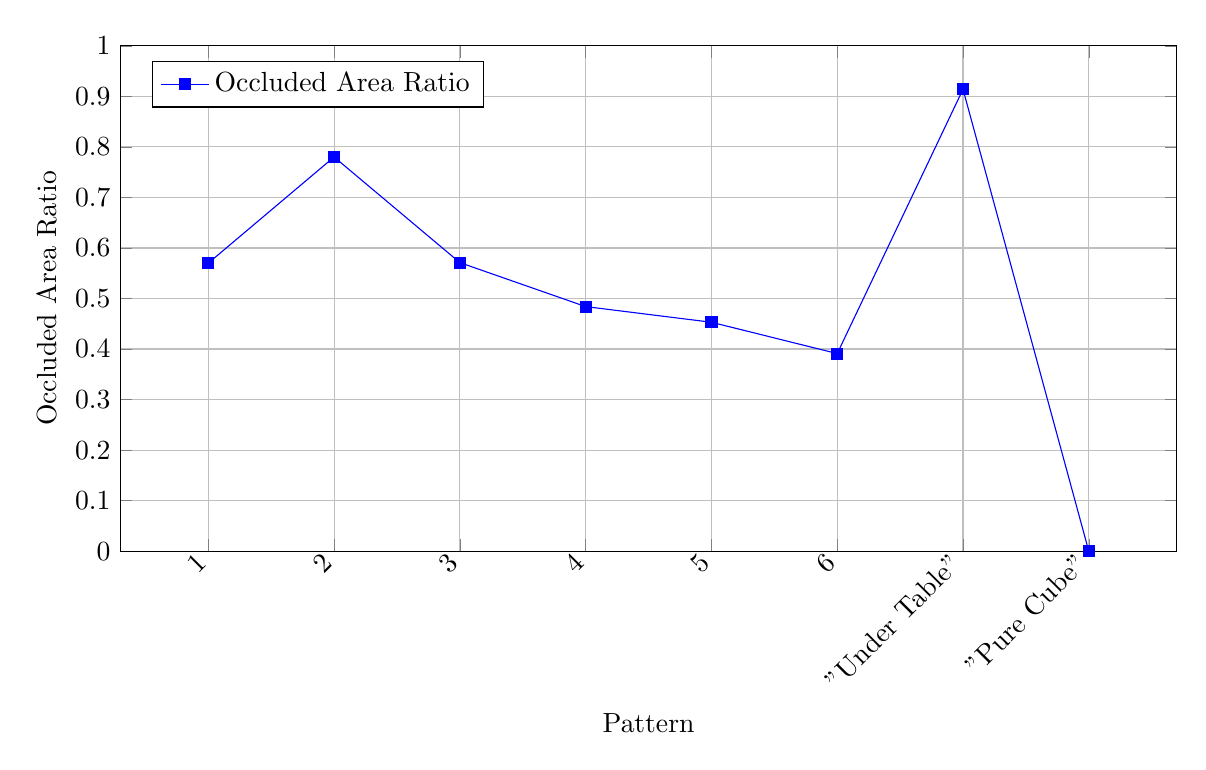
\begin{tikzpicture}
        \begin{axis}[
            xlabel=Pattern,
            ylabel=Occluded Area Ratio,
            xtick=data,
            xticklabels={1, 2, 3, 4, 5, 6, "Under Table", "Pure Cube"},
            x tick label style={rotate=45, anchor=east},
            ytick={0,0.1,...,1},
            ymin=0,
            ymax=1,
            grid=major,
            legend entries={Occluded Area Ratio},
            legend pos=north west,
            width=15cm,
            height=8cm,
        ]
        \addplot[
             mark=square*,
             blue
        ] coordinates {
            (1, 0.570)
            (2, 0.780)
            (3, 0.571)
            (4, 0.484)
            (5, 0.453)
            (6, 0.391)
            (7, 0.914)
            (8, 0.000)
        };
        \end{axis}
    \end{tikzpicture}
    \caption{Result of Ground Truth Mesh}
    \label{fig:result of gt mesh}
\end{figure}

\vspace{10pt}

Except for patterns we mentioned above, we also added 2 corner cases where in the first case we put one viewpoint right below the center as shown in Figure \ref{fig:corner case under table}. The only difference is that the Z-value of this viewpoint is equal to the minimal vertex of the scene. The center viewpoint is also shown since we want to display the relative position of the viewpoint used in corner case to it, but we don't consider it for computation. Based on its special position, most of the rays cast from samplings should be blocked by the table. The value \emph{0.914} can verify that in this case most samplings are occluded to this viewpoint, 

\begin{figure}[H]
    \centering
    \includegraphics*[width=0.8\textwidth]{figures/edge case-under table.png}
    \caption{Corner Case - Under Table}
    \label{fig:corner case under table}
\end{figure}

In the other corner case we change the scene to a pure cube where there is no clutter inside it. Thus, all samplings should be visible to a viewpoint inside the cube regardless of its position. The resulting visible sampling cloud is shown in Figure \ref{fig:corner case pure cube}. Our pipeline output the value \emph{0}, which can also validate the correctness of computation. 

\vspace{10pt}

\begin{figure}[H]
    \centering
    \includegraphics*[width=0.45\textwidth]{figures/cube with all samples.png}
    \caption{Corner Case - Pure Cube}
    \label{fig:corner case pure cube}
\end{figure}

Based on results presented above, we can take the \emph{Occluded Area Ratio} as a reliable metric to represent the occlusion level of a mesh.

\subsection{Estimated Mesh and Scanned Cloud} \label{subsec:estimate mesh and scanned cloud}

In this section we are going to compute occlusion level of estimated mesh and scanned point cloud respectively. 

\paragraph{Setup}

We prepare 2 original point clouds with name \emph{Conference Room 1} and \emph{Conference Room 2} respectively. For each of them, we estimate a mesh via \emph{GoCoPP}. Then for each mesh, we conduct the same workflow described in Section \ref{sec:compute occluded area ratio} to get \emph{Occluded Area Ratio}. The next step is to apply the computation pipeline of \emph{Boundary Ray Ratio} on scanned clouds, which will be generated by adopting the same patterns illustrated in Figure \ref{fig:pattern of viewpoints} to place spherical light sources as described in Section \ref{subsec:ray tracing point cloud scanning}.

\vspace{10pt}

Above workflow will be conducted for each scene 6 times as we would keep the same viewpoint strategy presented in Figure \ref{fig:pattern of viewpoints}, and each time we cast 10000 rays in the scene randomly for calculating \emph{Boundary Ray Ratio}.    

\paragraph{Conference Room 1} \label{par:conf1 result}

We present the visualization of the scene \emph{Conference Room 1} in each step. Figure \ref{fig:estimate mesh from conference room 1} shows the result of mesh estimation, where point clouds was transferred into a set of alpha-shape triangulated planar primitives.

\vspace{10pt}

To detect boundary ray we have to know each point's category in terms of boundary from scanned point cloud, where we use white color to represent boundary point and blue for non-boundary point as shown in Figure \ref{fig:conf1 0} (a). This boundary cloud is generated together with the ground truth scanned cloud displayed in Figure \ref{fig:conf1 0} (b). The resulting visualization will be displayed for clouds scanned under each pattern.

\vspace{30pt}

\begin{figure}[H]
    \centering
    \includegraphics*[width=1.0\textwidth]{figures/estimate conf1.png}
    \caption{Estimate Mesh from Conference Room 1}
    \label{fig:estimate mesh from conference room 1}
\end{figure}

\vspace{30pt}

In the end of this part, result of computation for \emph{Occluded Area Ratio} and \emph{Boundary Ray Ratio} is shown in Table \ref{tab:result of conference room 1} together with line graph illustrated in Figure \ref{fig:result of conference room 1}.

\vspace{30pt}

\begin{figure}[H]
    \centering
    \subfigure[Boundary]{\includegraphics[width=0.45\textwidth]{figures/conf1 0 b.png}}  \label{fig:conf1 0 b} \hfill
    \subfigure[Scanning]{\includegraphics[width=0.45\textwidth]{figures/conf1 0.png}} \label{fig:conf1 0 s}
    \caption{Boundary and Scanning of Conference Room 1 under Pattern 1 with 38372 Points}
    \label{fig:conf1 0}
\end{figure}

\vspace{80pt}

\begin{figure}[H]
    \centering
    \subfigure[Boundary]{\includegraphics[width=0.45\textwidth]{figures/conf1 1 b.png}}  \label{fig:conf1 b 1} \hfill
    \subfigure[Scanning]{\includegraphics[width=0.45\textwidth]{figures/conf1 1.png}} \label{fig:conf1 s 1}
    \caption{Boundary and Scanning of Conference Room 1 under Pattern 2 with 36152 Points}
    \label{fig:conf1 1}
\end{figure}

\vspace{80pt}

\begin{figure}[H]
    \centering
    \subfigure[Boundary]{\includegraphics[width=0.45\textwidth]{figures/conf1 2 b.png}}  \label{fig:conf1 b 2} \hfill
    \subfigure[Scanning]{\includegraphics[width=0.45\textwidth]{figures/conf1 2.png}} \label{fig:conf1 s 2}
    \caption{Boundary and Scanning of Conference Room 1 under Pattern 3 with 38834 Points}
    \label{fig:conf1 2}
\end{figure}

\begin{figure}[H]
    \centering
    \subfigure[Boundary]{\includegraphics[width=0.45\textwidth]{figures/conf1 4 b.png}}  \label{fig:conf1 b 4} \hfill
    \subfigure[Scanning]{\includegraphics[width=0.45\textwidth]{figures/conf1 4.png}} \label{fig:conf1 s 200 4}
    \caption{Boundary and Scanning of Conference Room 1 under Pattern 4 with 74524 Points}
    \label{fig:conf1 4}
\end{figure}

\vspace{80pt}

\begin{figure}[H]
    \centering
    \subfigure[Boundary]{\includegraphics[width=0.45\textwidth]{figures/conf1 5 b.png}}  \label{fig:conf1 b 5} \hfill
    \subfigure[Scanning]{\includegraphics[width=0.45\textwidth]{figures/conf1 5.png}} \label{fig:conf1 s 5}
    \caption{Boundary and Scanning of Conference Room 1 under Pattern 5 with 77206 Points}
    \label{fig:conf1 5}
\end{figure}

\begin{figure}[H]
    \centering
    \subfigure[Boundary]{\includegraphics[width=0.45\textwidth]{figures/conf1 6 b.png}}  \label{fig:conf1 b 6} \hfill
    \subfigure[Scanning]{\includegraphics[width=0.45\textwidth]{figures/conf1 6.png}} \label{fig:conf1 s 6}
    \caption{Boundary and Scanning of Conference Room 1 under Pattern 6 with 113358 Points}
    \label{fig:conf1 6}
\end{figure}

\begin{table}[H]
    \centering
    \begin{tabular}{|c|c|c|}
        \hline
        \textbf{Pattern} & \textbf{Occluded Area Ratio} & \textbf{Boundary Ray Ratio} \\
        \hline
        1 & 0.291 & 0.248 \\
        2 & 0.178 & 0.214 \\
		3 & 0.290 & 0.332 \\
		4 & 0.109 & 0.173 \\
        5 & 0.153 & 0.194 \\
        6 & 0.071 & 0.165 \\
        \hline
    \end{tabular}
    \caption{Result of Conference Room 1}
    \label{tab:result of conference room 1}
\end{table}

The result shows that as the number of viewpoints increase, the \emph{Occluded Area Ratio} decrease. There are 2 viewpoints in both pattern 4 and 5, thus the increase of data in pattern 5 is not against our conclusion. Values of \emph{Boundary Ray Ratio} describe the same tendency, and they do not differ too much from data in \emph{Occluded Area Ratio}. Therefore, based on these results we consider \emph{Boundary Ray Ratio} as a reliable metric to represent the occlusion level of the scene presented by point cloud \emph{Conference Room 1}.       

\begin{figure}[H]
    \centering
    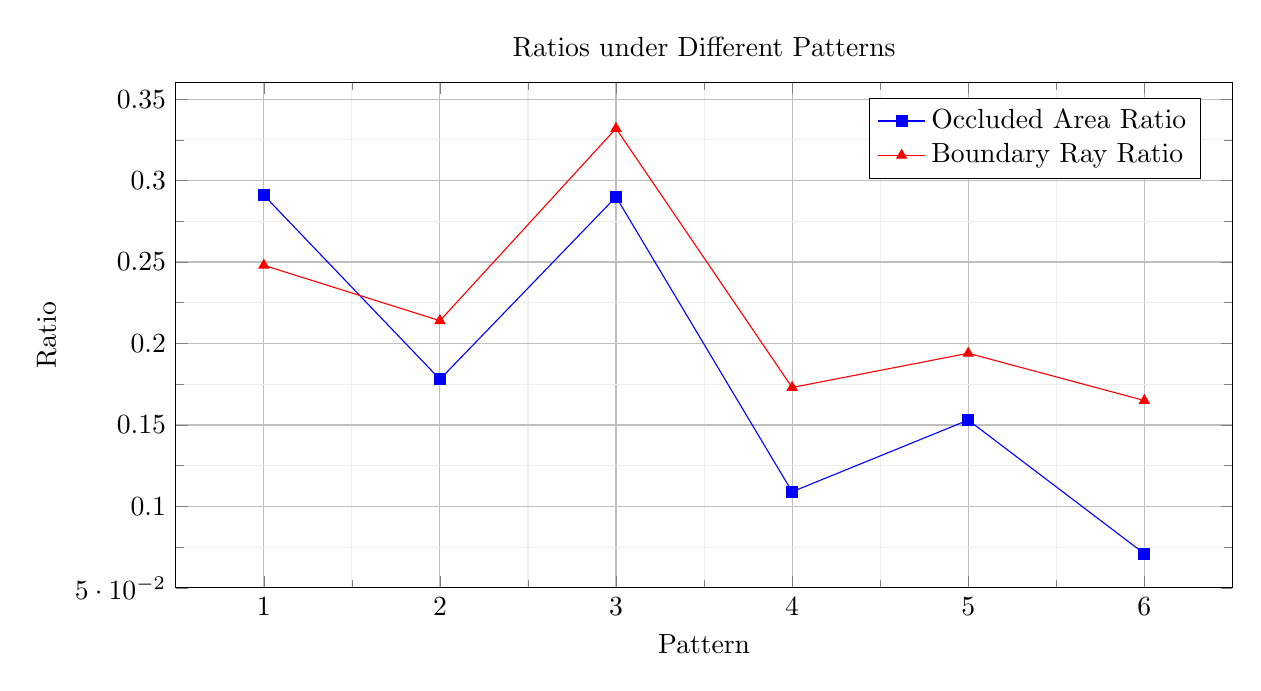
\begin{tikzpicture}
        \begin{axis}[
            title={Ratios under Different Patterns},
            xlabel={Pattern},
            ylabel={Ratio},
            grid=both,
            minor tick num=1,
            major grid style={lightgray},
            minor grid style={lightgray!25},
            legend pos=north east,
            legend style={cells={anchor=west}},
            xtick=data,  % Only show integer values on the x axis
            xticklabels={1,2,3,4,5,6},  % Specify the labels for the x axis
            ymin=0.05,
            width=15cm,
            height=8cm
        ]
        
        % Occluded Area Ratio Line
        \addplot[color=blue,mark=square*] coordinates {
            (1, 0.291)
            (2, 0.178)
            (3, 0.290)
            (4, 0.109)
            (5, 0.153)
            (6, 0.071)
        };
        \addlegendentry{Occluded Area Ratio}
        
        % Boundary Ray Ratio Line
        \addplot[color=red,mark=triangle*] coordinates {
            (1, 0.248)
            (2, 0.214)
            (3, 0.332)
            (4, 0.173)
            (5, 0.194)
            (6, 0.165)
        };
        \addlegendentry{Boundary Ray Ratio}

        \end{axis}
    \end{tikzpicture}
    \caption{Result of Conference Room 1}
    \label{fig:result of conference room 1}
\end{figure}

\vspace{30pt}

\paragraph{Conference Room 2}

The resulting mesh estimation is shown in Figure \ref{fig:estimate mesh from conference room 2}. Then we present the visualization of scanned point cloud together with its boundary cloud. The workflow here is the same as explained in \ref{par:conf1 result} and conducted with same patterns displayed in Figure \ref{fig:pattern of viewpoints}. Results are shown in the end of the part in Table \ref{tab:result of conference room 2} and Figure \ref{fig:result of conference room 2}.

\vspace{10pt}

\begin{figure}[H]
    \centering
    \includegraphics*[width=1.0\textwidth]{figures/estimate conf2.png}
    \caption{Estimate Mesh from Conference Room 2}
    \label{fig:estimate mesh from conference room 2}
\end{figure}

\begin{figure}[H]
    \centering
    \subfigure[Boundary]{\includegraphics[width=0.45\textwidth]{figures/conf2 0 b.png}}  \label{fig:conf2 b 0} \hfill
    \subfigure[Scanning]{\includegraphics[width=0.45\textwidth]{figures/conf2 0.png}} \label{fig:conf2 s 0}
    \caption{Boundary and Scanning of Conference Room 2 under Pattern 1 with 36742 Points}
    \label{fig:conf2 0}
\end{figure}

\begin{figure}[H]
    \centering
    \subfigure[Boundary]{\includegraphics[width=0.45\textwidth]{figures/conf2 1 b.png}}  \label{fig:conf2 b 1} \hfill
    \subfigure[Scanning]{\includegraphics[width=0.45\textwidth]{figures/conf2 1.png}} \label{fig:conf2 s 1}
    \caption{Boundary and Scanning of Conference Room 2 under Pattern 2 with 34270 Points}
    \label{fig:conf2 1}
\end{figure}

\begin{figure}[H]
    \centering
    \subfigure[Boundary]{\includegraphics[width=0.45\textwidth]{figures/conf2 2 b.png}}  \label{fig:conf2 b 2} \hfill
    \subfigure[Scanning]{\includegraphics[width=0.45\textwidth]{figures/conf2 2.png}} \label{fig:conf2 s 2}
    \caption{Boundary and Scanning of Conference Room 2 under Pattern 3 with 35260 Points}
    \label{fig:conf2 2}
\end{figure}

\begin{figure}[H]
    \centering
    \subfigure[Boundary]{\includegraphics[width=0.45\textwidth]{figures/conf2 4 b.png}}  \label{fig:conf2 b 4} \hfill
    \subfigure[Scanning]{\includegraphics[width=0.45\textwidth]{figures/conf2 4.png}} \label{fig:conf2 s 4}
    \caption{Boundary and Scanning of Conference Room 2 under Pattern 4 with 71012 Points}
    \label{fig:conf2 4}
\end{figure}

\begin{figure}[H]
    \centering
    \subfigure[Boundary]{\includegraphics[width=0.45\textwidth]{figures/conf2 5 b.png}}  \label{fig:conf2 b 5} \hfill
    \subfigure[Scanning]{\includegraphics[width=0.45\textwidth]{figures/conf2 5.png}} \label{fig:conf2 s 5}
    \caption{Boundary and Scanning of Conference Room 2 under Pattern 5 with 72002 Points}
    \label{fig:conf2 5}
\end{figure}

\begin{figure}[H]
    \centering
    \subfigure[Boundary]{\includegraphics[width=0.45\textwidth]{figures/conf2 6 b.png}}  \label{fig:conf2 b 6} \hfill
    \subfigure[Scanning]{\includegraphics[width=0.45\textwidth]{figures/conf2 6.png}} \label{fig:conf2 s 6}
    \caption{Boundary and Scanning of Conference Room 2 under Pattern 6 with 106272 Points}
    \label{fig:conf2 6}
\end{figure}

\begin{table}[H]
    \centering
    \begin{tabular}{|c|c|c|}
        \hline
        \textbf{Pattern} & \textbf{Occluded Area Ratio} & \textbf{Boundary Ray Ratio} \\
        \hline
        1 & 0.371 & 0.319 \\
        2 & 0.525 & 0.473 \\
        3 & 0.313 & 0.321 \\
        4 & 0.294 & 0.282 \\
		5 & 0.264 & 0.265 \\
		6 & 0.218 & 0.223 \\
        \hline
    \end{tabular}
    \caption{Result of Conference Room 2}
    \label{tab:result of conference room 2}
\end{table}

Both ratios display the same trend and also present a minor difference on value. Thus we can conclude that \emph{Boundary Ray Ratio} is able to assess the occlusion level of \emph{Conference Room 2}.

\begin{figure}[H]
    \centering
    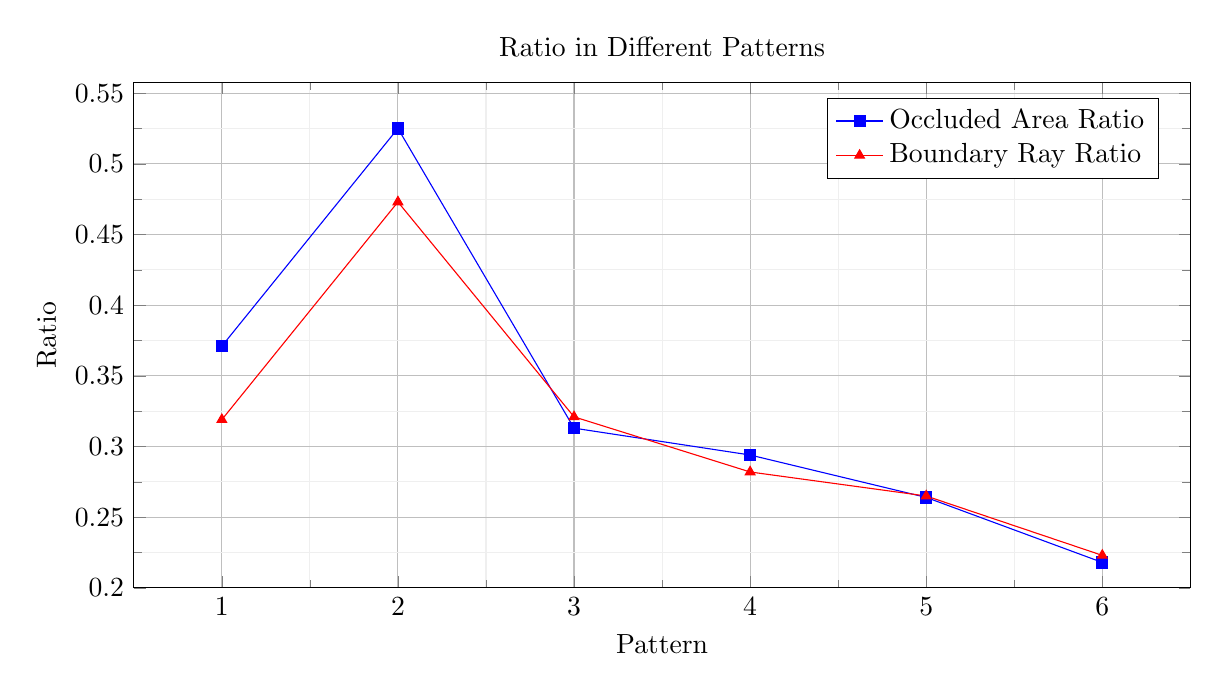
\begin{tikzpicture}
        \begin{axis}[
            title={Ratio in Different Patterns},
            xlabel={Pattern},
            ylabel={Ratio},
            grid=both,
            minor tick num=1,
            major grid style={lightgray},
            minor grid style={lightgray!25},
            legend pos=north east,
            legend style={cells={anchor=west}},
            xtick=data,  % Only show integer values on the x axis
            xticklabels={1,2,3,4,5,6},  % Specify the labels for the x axis
            ymin=0.2,
            width=15cm,
            height=8cm
        ]
        
        % Occluded Area Ratio Line
        \addplot[color=blue,mark=square*] coordinates {
            (1, 0.371)
            (2, 0.525)
            (3, 0.313)
            (4, 0.294)
            (5, 0.264)
            (6, 0.218)
        };
        \addlegendentry{Occluded Area Ratio}
        
        % Boundary Ray Ratio Line
        \addplot[color=red,mark=triangle*] coordinates {
            (1, 0.319)
            (2, 0.473)
            (3, 0.321)
            (4, 0.282)
            (5, 0.265)
            (6, 0.223)
        };
        \addlegendentry{Boundary Ray Ratio}

        \end{axis}
    \end{tikzpicture}
    \caption{Result of Conference Room 2}
    \label{fig:result of conference room 2}
\end{figure}


In this section we conducted 2 experiments to compute and compare occlusion level for different scenes. The result proves that \emph{Boundary Ray Ratio} can be applied for computation in subsequent experiments.

\section{Correlation} \label{sec:correlation}

The major task in this part is to find correlation between occlusion level and performance of segmentation. Due to the difference in terms of complexity and structure of the 2 scenes, it is obviously not a feasible way to directly compare the metrics of them. Thus, We apply scanned point clouds generated in previous experiment as input data to \emph{Minkowski Engine} for semantic segmentation. In the final step, we calculate evaluation metrics for each segmented cloud. With occlusion level and result of evaluation metrics of this data set, we may correlate them and analyze the impact of occlusion on semantic segmentation. The comparison should be done between data generated from the same scene.

\subsection{Setup}

To generate occluded point cloud, we place spherical light sources in different locations of the scene. Each light source cast a set of rays based on the result of halton sampling on its surface. We will then record the point hit by rays for the first time to generate occluded point cloud.

\vspace{10pt}

We apply the same pattern of placement illustrated in Figure \ref{fig:pattern of viewpoints} to place our sphere lights in the scene. 

\vspace{10pt}

Point cloud with estimated semantic information is then generated for each occluded point cloud via \emph{Minkowski Engine}. We calculate values of evaluation metrics in a pair-wise manner.


\subsection{Results}

In this part, we display visualization for each pair of clouds which includes one occluded cloud with ground truth RGB information and one cloud with semantic label represented by specific colors. In the end of each part, output of the computational pipeline will be shown in tables and graphs where we can compare data more conveniently.

\paragraph{Conference Room 1} \label{par:corre conf1}

We first exhibit visual output of scanned point cloud again and then its corresponding segmentation of \emph{Conference Room 1}.

\begin{figure}[H]
    \centering
    \subfigure[Scanning]{\includegraphics[width=0.42\textwidth]{figures/conf1 0.png}}  \label{fig:conf1 0 occluded} \hfill
    \subfigure[Segmentation]{\includegraphics[width=0.42\textwidth]{figures/conf1 0 seg.png}} \label{fig:conf1 0 seg}
    \caption{Scanning and Corresponding Segmentation under Pattern 1 of Conference Room 1}
    \label{fig:conf1 0 occ and seg}
\end{figure}

\begin{figure}[H]
    \centering
    \subfigure[Scanning]{\includegraphics[width=0.42\textwidth]{figures/conf1 1.png}}  \label{fig:conf1 1 occluded} \hfill
    \subfigure[Segmentation]{\includegraphics[width=0.42\textwidth]{figures/conf1 1 seg.png}} \label{fig:conf1 1 seg}
    \caption{Scanning and Corresponding Segmentation under Pattern 2 of Conference Room 1}
    \label{fig:conf1 1 occ and seg}
\end{figure}


\begin{figure}[H]
    \centering
    \subfigure[Scanning]{\includegraphics[width=0.42\textwidth]{figures/conf1 2.png}}  \label{fig:conf1 2 occluded} \hfill
    \subfigure[Segmentation]{\includegraphics[width=0.42\textwidth]{figures/conf1 2 seg.png}} \label{fig:conf1 2 seg}
    \caption{Scanning and Corresponding Segmentation under Pattern 3 of Conference Room 1}
    \label{fig:conf1 2 occ and seg}
\end{figure}

\vspace{80pt}

\begin{figure}[H]
    \centering
    \subfigure[Scanning]{\includegraphics[width=0.42\textwidth]{figures/conf1 4.png}}  \label{fig:conf1 4 occluded} \hfill
    \subfigure[Segmentation]{\includegraphics[width=0.42\textwidth]{figures/conf1 4 seg.png}} \label{fig:conf1 4 seg}
    \caption{Scanning and Corresponding Segmentation under Pattern 4 of Conference Room 1}
    \label{fig:conf1 4 occ and seg}
\end{figure}

\begin{figure}[H]
    \centering
    \subfigure[Scanning]{\includegraphics[width=0.42\textwidth]{figures/conf1 5.png}}  \label{fig:conf1 5 occluded} \hfill
    \subfigure[Segmentation]{\includegraphics[width=0.42\textwidth]{figures/conf1 5 seg.png}} \label{fig:conf1 5 seg}
    \caption{Scanning and Corresponding Segmentation under Pattern 5 of Conference Room 1}
    \label{fig:conf1 5 occ and seg}
\end{figure}

\begin{figure}[H]
    \centering
    \subfigure[Scanning]{\includegraphics[width=0.42\textwidth]{figures/conf1 6.png}}  \label{fig:conf1 6 occluded} \hfill
    \subfigure[Segmentation]{\includegraphics[width=0.42\textwidth]{figures/conf1 6 seg.png}} \label{fig:conf1 6 seg}
    \caption{Scanning and Corresponding Segmentation under Pattern 6 of Conference Room 1}
    \label{fig:conf1 6 occ and seg}
\end{figure}

The result is shown below in Table \ref{tab:evaluation metrics of conference room 1} and Figure \ref{fig:evaluation metrics of conference room 1}.

\begin{table}[H]
    \centering
    \begin{tabular}{|c|c|c|}
        \hline
        Pattern & Occlusion & F1 Score \\
        \hline
        1 & 0.248 & 0.826 \\
        2 & 0.214 & 0.887 \\
        3 & 0.332 & 0.680 \\
        4 & 0.173 & 0.886 \\
        5 & 0.194 & 0.737 \\
        6 & 0.165 & 0.807 \\
        \hline
    \end{tabular}
    \caption{Evaluation Metrics of Conference Room 1}
    \label{tab:evaluation metrics of conference room 1}
\end{table}

From the graph we can see opposite trends between occlusion level and evaluation metrics. This indicates an inversely proportional relationship. If we compare data of clouds under different patterns pair-wisely, the negative correlation does not always hold. For example, occlusion level of cloud under pattern 4 is higher than the value in pattern 6, but F1 score in pattern 4 is still higher. Based on that, we conclude that the occlusion level and performance of semantic segmentation are inversely proportional related to each other in terms of \emph{Conference Room 1}.

\begin{figure}[H]
    \centering
    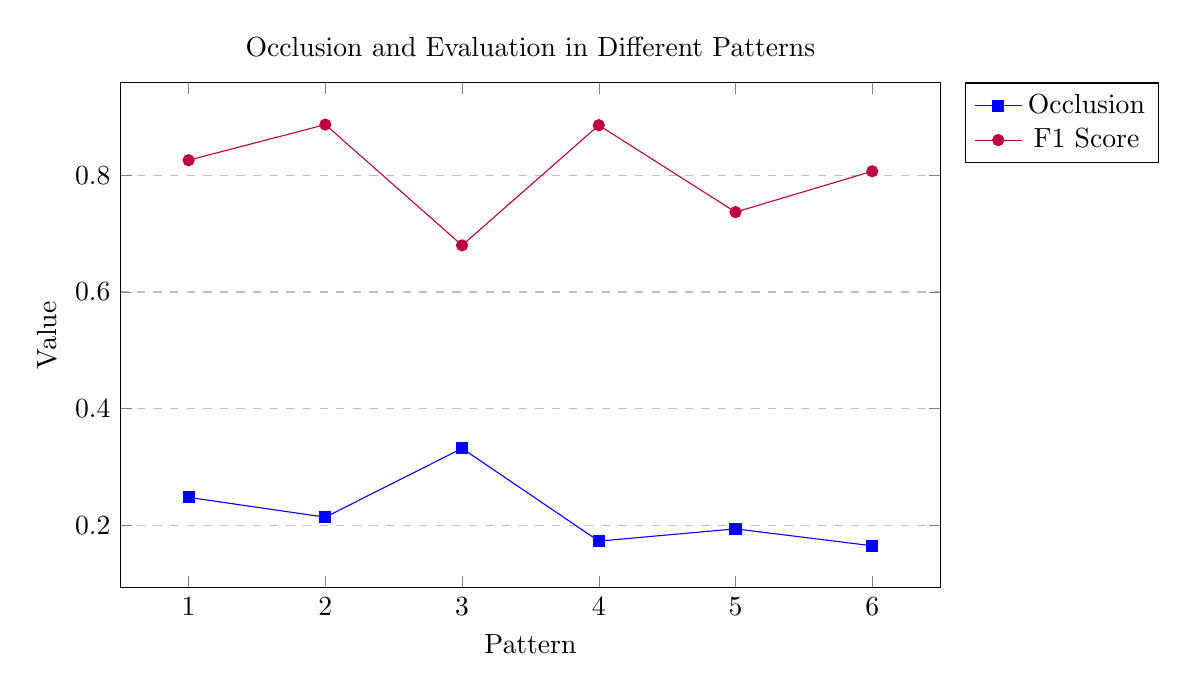
\begin{tikzpicture}
    \begin{axis}[
        title={Occlusion and Evaluation in Different Patterns},
        xlabel={Pattern},
        ylabel={Value},
        legend pos=outer north east,
        ymajorgrids=true,
        grid style=dashed,
        xtick=data,
        symbolic x coords={1,2,3,4,5,6},
        width=12cm,
        height=8cm,
    ]
    
    \addplot[mark=square*,blue] coordinates {
        (1, 0.248)
        (2, 0.214)
        (3, 0.332)
        (4, 0.173)
        (5, 0.194)
        (6, 0.165)
    };
    \addlegendentry{Occlusion}
    
    \addplot[mark=*,purple] coordinates {
        (1, 0.826)
        (2, 0.887)
        (3, 0.680)
        (4, 0.886)
        (5, 0.737)
        (6, 0.807)
    };
    \addlegendentry{F1 Score}
    
    \end{axis}
    \end{tikzpicture}
    \caption{Evaluation Result of Conference Room 1}
    \label{fig:evaluation metrics of conference room 1}
\end{figure}

\vspace{30pt}

\paragraph{Conference Room 2}

We apply same workflow as described in \emph{Conference Room 1} to present our results.

\begin{figure}[H]
    \centering
    \subfigure[Scanning]{\includegraphics[width=0.45\textwidth]{figures/conf2 0.png}}  \label{fig:conf2 0 occluded} \hfill
    \subfigure[Segmentation]{\includegraphics[width=0.45\textwidth]{figures/conf2 0 seg.png}} \label{fig:conf2 0 seg}
    \caption{Scanning and Corresponding Segmentation under Pattern 1 of Conference Room 2}
    \label{fig:conf2 0 occ and seg}
\end{figure}

\begin{figure}[H]
    \centering
    \subfigure[Scanning]{\includegraphics[width=0.45\textwidth]{figures/conf2 1.png}}  \label{fig:conf2 1 occluded} \hfill
    \subfigure[Segmentation]{\includegraphics[width=0.45\textwidth]{figures/conf2 1 seg.png}} \label{fig:conf2 1 seg}
    \caption{Scanning and Corresponding Segmentation under Pattern 2 of Conference Room 2}
    \label{fig:conf2 1 occ and seg}
\end{figure}

\begin{figure}[H]
    \centering
    \subfigure[Scanning]{\includegraphics[width=0.45\textwidth]{figures/conf2 2.png}}  \label{fig:conf2 2 occluded} \hfill
    \subfigure[Segmentation]{\includegraphics[width=0.45\textwidth]{figures/conf2 2 seg.png}} \label{fig:conf2 2 seg}
    \caption{Scanning and Corresponding Segmentation under Pattern 3 of Conference Room 2}
    \label{fig:conf2 2 occ and seg}
\end{figure}

\begin{figure}[H]
    \centering
    \subfigure[Scanning]{\includegraphics[width=0.45\textwidth]{figures/conf2 4.png}}  \label{fig:conf2 4 occluded} \hfill
    \subfigure[Segmentation]{\includegraphics[width=0.45\textwidth]{figures/conf2 4 seg.png}} \label{fig:conf2 4 seg}
    \caption{Scanning and Corresponding Segmentation  under Pattern 4 of Conference Room 2}
    \label{fig:conf2 4 occ and seg}
\end{figure}

\begin{figure}[H]
    \centering
    \subfigure[Scanning]{\includegraphics[width=0.45\textwidth]{figures/conf2 5.png}}  \label{fig:conf2 5 occluded} \hfill
    \subfigure[Segmentation]{\includegraphics[width=0.45\textwidth]{figures/conf2 5 seg.png}} \label{fig:conf2 5 seg}
    \caption{Scanning and Corresponding Segmentation under Pattern 5 of Conference Room 2}
    \label{fig:conf2 5 occ and seg}
\end{figure}

\begin{figure}[H]
    \centering
    \subfigure[Scanning]{\includegraphics[width=0.45\textwidth]{figures/conf2 6.png}}  \label{fig:conf2 6 occluded} \hfill
    \subfigure[Segmentation]{\includegraphics[width=0.45\textwidth]{figures/conf2 6 seg.png}} \label{fig:conf2 6 seg}
    \caption{Scanning and Corresponding Segmentation under Pattern 6 of Conference Room 2}
    \label{fig:conf2 6 occ and seg}
\end{figure}

The result is shown in Table \ref{tab:evaluation metrics of conference room 2} and Figure \ref{fig:evaluation metrics of conference room 2}.

\begin{table}[H]
    \centering
    \begin{tabular}{|c|c|c|}
        \hline
        Pattern & Occlusion & F1 Score \\
        \hline
        1 & 0.319 & 0.765 \\
        2 & 0.473 & 0.888 \\
        3 & 0.321 & 0.772 \\
        4 & 0.282 & 0.858 \\
        5 & 0.265 & 0.797 \\
        6 & 0.223 & 0.837 \\
        \hline
    \end{tabular}
    \caption{Occlusion and Evaluation of Conference Room 2}
    \label{tab:evaluation metrics of conference room 2}
\end{table}

The results in pattern 1, 2 and 3 show the same trends as opposed to the result of \emph{Conference Room 1}. If we compare data in other patterns pair-wisely,  both positive and negative relationships can be found. Hence, we came to the conclusion that no obvious correlation can be found between occlusion level and performance of semantic segmentation in terms of \emph{Conference Room 2}.

\begin{figure}[H]
    \centering
    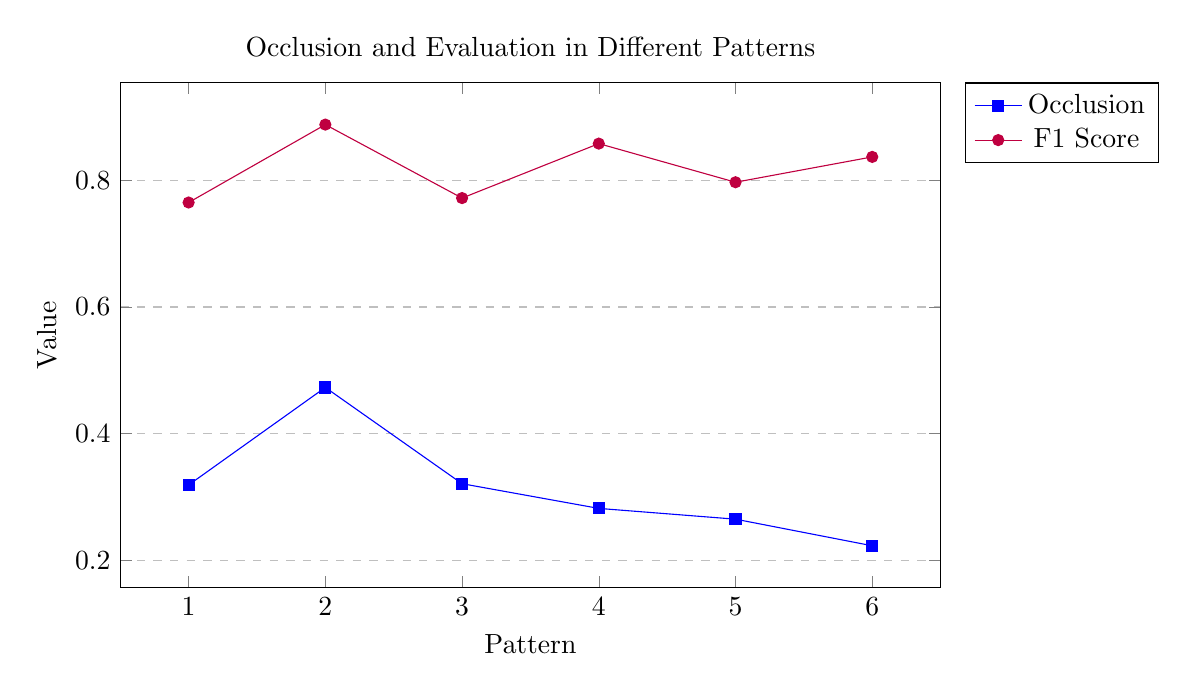
\begin{tikzpicture}
    \begin{axis}[
        title={Occlusion and Evaluation in Different Patterns},
        xlabel={Pattern},
        ylabel={Value},
        legend pos=outer north east,
        ymajorgrids=true,
        grid style=dashed,
        xtick=data,
        symbolic x coords={1,2,3,4,5,6},
        width=12cm,
        height=8cm,
    ]
    
    \addplot[mark=square*,blue] coordinates {
        (1, 0.319)
        (2, 0.473)
        (3, 0.321)
        (4, 0.282)
        (5, 0.265)
        (6, 0.223)
    };
    \addlegendentry{Occlusion}
    
    \addplot[mark=*,purple] coordinates {
        (1, 0.765)
        (2, 0.888)
        (3, 0.772)
        (4, 0.858)
        (5, 0.797)
        (6, 0.837)
    };
    \addlegendentry{F1 Score}
    
    \end{axis}
    \end{tikzpicture}
    \caption{Occlusion and Evaluation of Conference Room 2}
    \label{fig:evaluation metrics of conference room 2}
\end{figure}


%=====================================================================
\chapter{Conclusion and Discussion} \label{chp:conclusion}
%=====================================================================

\section{Conclusion} \label{sec:conclusion}

Semantic segmentation achieved through \emph{Minkowski Engine} shows a good understanding on classification of structure and objects of the point cloud based indoor scene. But the accuracy of the output still needs to be improved in order to extend the application of semantic segmentation. Hence, in this bachelor thesis we focus on occlusion, which is a common feature to represent the loss of information of point cloud acquired by scanning, to investigate its impact on the performance of semantic segmentation. We first proposed the metric \emph{occluded area ratio} to reflect the occlusion level of mesh. Then we extend this concept to point cloud and proposed another metric \emph{boundary ray ratio}. Through the comparison of the 2 ratios of the same scene in Section \ref{subsec:estimate mesh and scanned cloud} we came to the conclusion that \emph{boundary ray ratio} is a reliable metric to estimate occlusion level of a point cloud. Based on that we applied this metric in our experiments to estimate how much the set of scanned point clouds are occluded and compare the output with the result of evaluation metric \emph{F1 score}. From the results described in Section \ref{sec:correlation}, we found that in the scene \emph{conference room 1} there exists an inversely proportional relationship between occlusion level and performance of semantic segmentation, while in \emph{Conference Room 2} there is no obvious correlation can be found. 

\vspace{10pt}

It is worth to mention some edge cases such as the cloud scanned under pattern 2 of \emph{conference room 2} shown in Figure \ref{fig:conf2 1 occ and seg}, where the cloud has the largest loss of information but scores highest on performance. If we inspect this cloud carefully, we can notice that despite the significant incompleteness of the whole scene, the region close to the corner exhibits a dense state, thus the segmentation method might have better understanding there due to high richness of structural information. This indicates that the performance is also affected by structure of point cloud and density of points in certain region. Therefore, occlusion alone is not enough to affect the result of semantic segmentation. It is critical to consider additional metrics to obtain a better evaluation. Other influential factors may include the complexity of the scenes being segmented, variations in placement of light sources, and the diversity of the interior items. Moreover, spatial relationship between different objects and structures may affect segmentation method's understanding on point cloud. According to these findings, we came to the conclusion that occlusion level of point cloud has limited impact on its performance of semantic segmentation.

\vspace{10pt}

\section{Discussion}

\subsection{Limitation} \label{subsec:limit}


Although the reliability of the metric for estimating occlusion level has been proven, it is not computing the real occlusion of point cloud. Our way of estimation is achieved through random rays intersecting boundary points, which is highly dependent on the exterior structure of the scene. Due to the limited diversity of data used in our experiments, we cannot guarantee that our metric will remain effective on more complex structures.

\vspace{10pt}

\subsection{Future Work} \label{subsec:futurework}

Some future work can be done for improvements. More data with different structures and complexities can be used in experiments to improve robustness and reliability of occlusion metrics. The development of more comprehensive metrics for evaluating occlusion levels should be a priority, with a focus on considering the complex interrelations of elements within the scene. This could alternatively be done by proposing an evaluation system for assessing the completeness of the scene, where influential factors regarding semantic segmentation are assigned with certain weights for  computation.

By addressing these aspects, we can expect advancements in devising better metrics or system to evaluate factors that may influence semantic segmentation.



%-------------------------------------------------------------------------------------------------------------------------
\chapter{Acknowledgements} \label{chp:acknowledgements}

I would like to extend my heartfelt gratitude to the Visualization and MultiMedia Laboratory for providing me with the opportunity to undertake this challenging yet fascinating topic. I would also express my sincere appreciation to Prof. Dr. Renato Pajarola for the continual assistance and invaluable suggestions throughout the entire process. Special thanks go to Lizeth J. Fuentes Perez, whose detailed guidance and dedication to spending regular time discussing various aspects of this project have been instrumental. Lastly, I have to thank my family and friends, your support has allowed me to concentrate fully on completing this project. 

\bibliographystyle{alpha}
\bibliography{references}
\end{document}
